\documentclass[12pt,letterpaper,oneside]{book}
\usepackage{../../afitStyleFiles/afitThesis}
\usepackage[nolist]{acronym}
\usepackage{todo}
\usepackage{tabu}
\usepackage{makecell}
\graphicspath{{../../Figures/}}
%% myFigures.tex
% A common file to store all figure definitions
%
% In preparing your thesis, one of the first things you should do is
% organize your figures.  Then, one of the last things you'll do is
% reorder your figures so they display where you want them to in the
% text.  Organizing figure definitions in a common files helps:
%
%   1. Write new figures using earlier examples.
%
%   2.  Isolate code and minimize the risk of introducing bugs in the
%   final editing process.  Trust me, moving around just one line of
%   code is easier.
%
%   3.  Reuse figures in other papers.  <=== the best reason!
%
% Note command names can not include numbers and special characters.
%
% To make the file more searchable, use naming conventions that map
% the graphics filename labSetup.jpg to the command name \figlabSetup to the
% figure label fig:labSetup.
% 

\newcommand{\figMpduFormat}{
	\begin{figure}[H]
		\begin{center}
			\makebox[\textwidth][c]{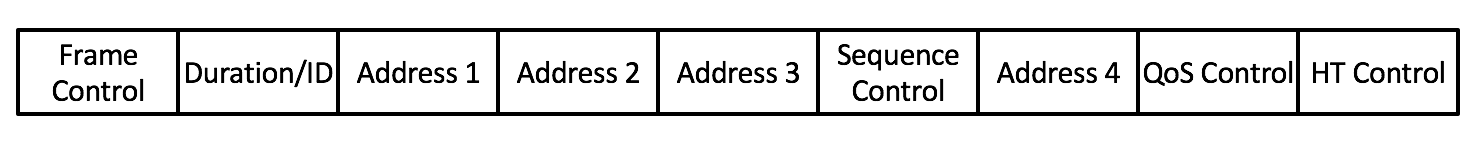
\includegraphics[width=\linewidth]{macHeader}}
			\caption{\ac{MPDU} format when using \ac{WPA}-2 \cite{802.11}}
			\label{fig:MpduFormat}
		\end{center}
		\vspace{-0.2 in}
	\end{figure}
}

\newcommand{\figMacHeader}{
	\begin{figure}[H]
		\begin{center}
			\makebox[\textwidth][c]{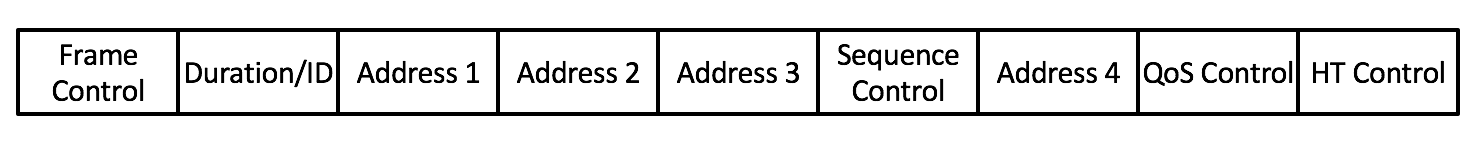
\includegraphics[width=\linewidth]{macHeader}}
			\caption{\ac{MAC} Header Frame Format \cite{802.11}}
			\label{fig:MacHeader}
		\end{center}
		\vspace{-0.2 in}
	\end{figure}
}

\newcommand{\figArchitecture}{\begin{figure}[H]
	\begin{center}
		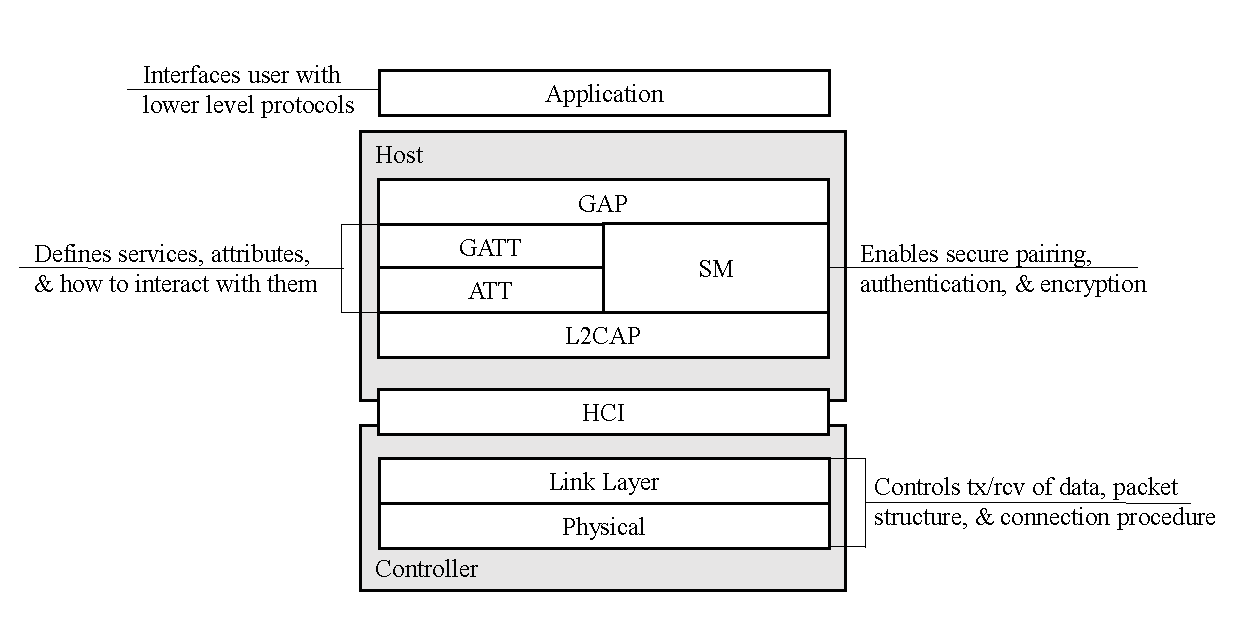
\includegraphics[width=4in]{architecture}
		\caption{The Bluetooth Low Energy Architecture}
		\label{fig:Architecture}
	\end{center}
	\vspace{-0.2 in}
\end{figure}
}

\newcommand{\figConnection}{\begin{figure}[H]
	\begin{center}
		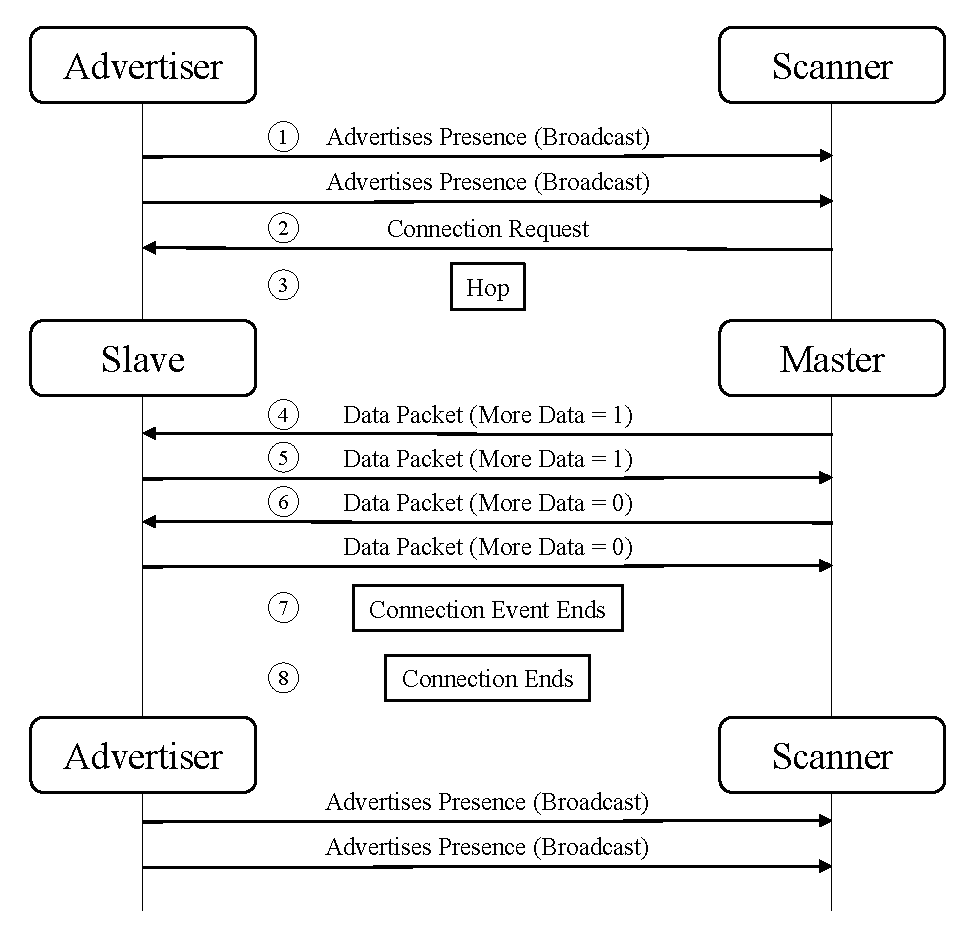
\includegraphics[width=4in]{connectionProcess}
		\caption{The \ac{BLE} Connection Process}
		\label{fig:Connection}
	\end{center}
	\vspace{-0.2 in}
\end{figure}
}

\newcommand{\figScanning}{\begin{figure}[H]
		\begin{center}
			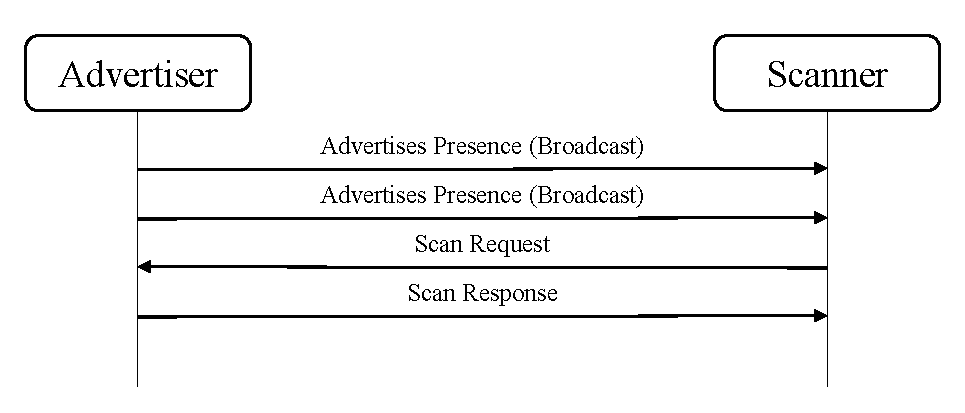
\includegraphics[width=4in]{activeScanning}
			\caption{Active Scanning Process}
			\label{fig:Scanning}
		\end{center}
		\vspace{-0.2 in}
	\end{figure}
}

\newcommand{\figChannel}{
	\begin{figure}[H]
		\begin{center}
			\includegraphics[width=5in]{channelMap}
			\caption{Bluetooth Low Energy channel mapping; darker channels represent advertisement channels}
			\label{fig:Channel}
		\end{center}
		\vspace{-0.2 in}
	\end{figure}
}

\newcommand{\figAccessPoint}{
	\begin{figure}[H]
		\begin{center}
			\makebox[\textwidth][c]{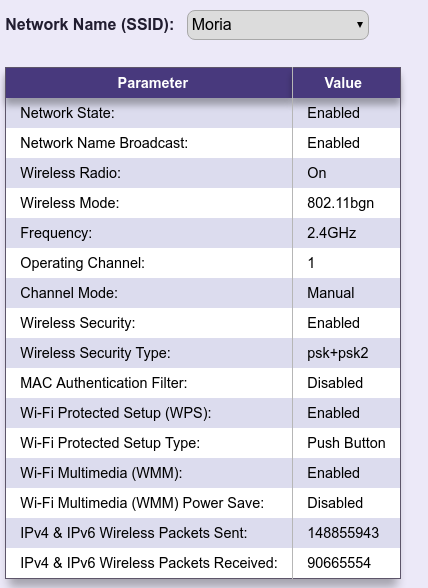
\includegraphics[width=2.5in]{accessPoint}}
			\caption{Prancing Pony Access Point Settings}
			\label{fig:AccessPoint}
		\end{center}
		\vspace{-0.2 in}
	\end{figure}
}

\newcommand{\figSystemDiagram}{
	\begin{figure}[h!]
		\begin{center}
			\centering
			\makebox[\textwidth][c]{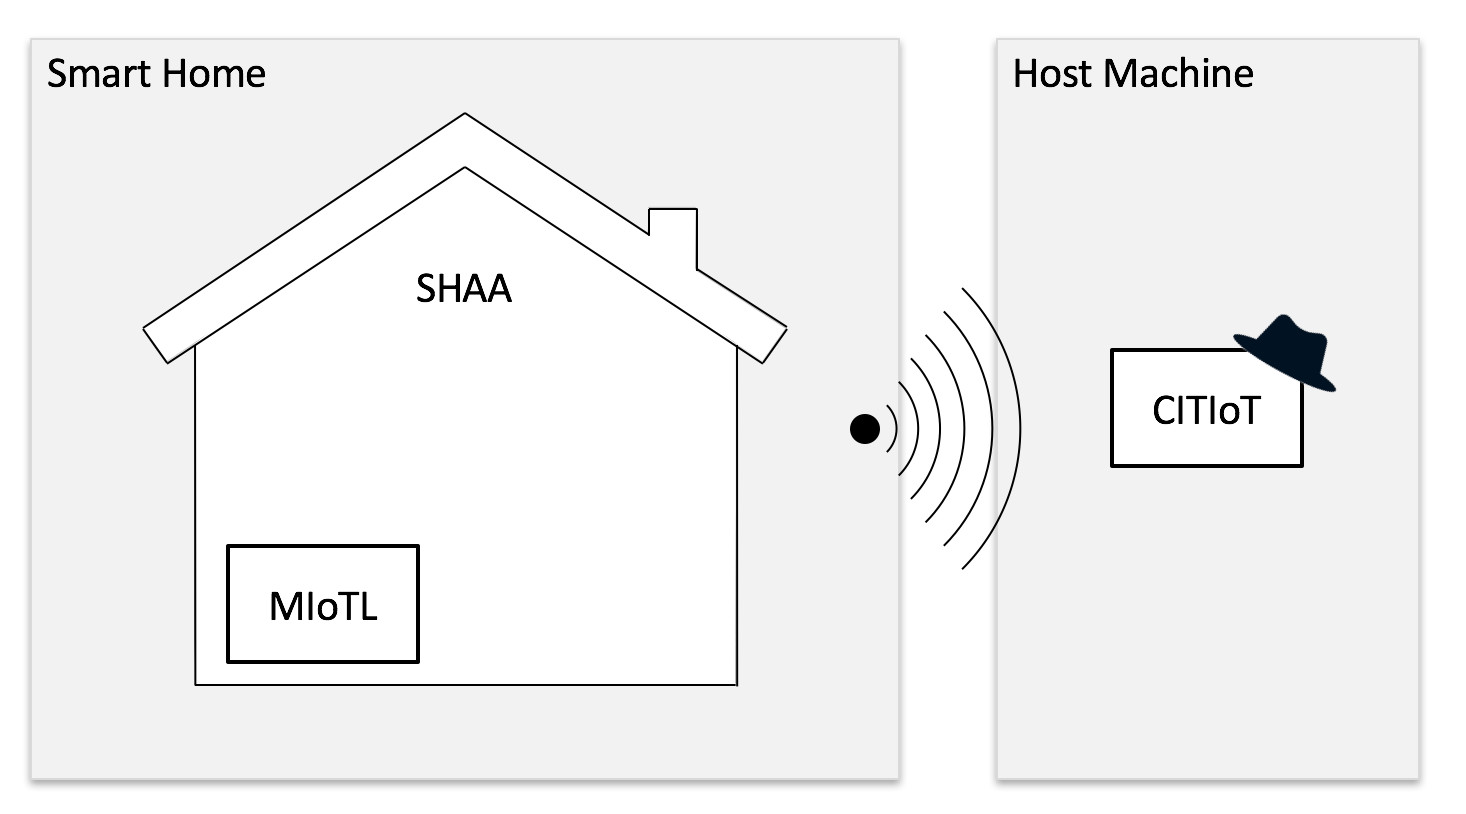
\includegraphics[width=4in]{systemDiagram}}
			\caption{Overall system diagram}
			\label{fig:SystemDiagram}
		\end{center}
		\vspace{-0.2 in}
	\end{figure}
}

\newcommand{\figShaaDiagram}{
	\begin{figure*}[h!]
		\begin{center}
			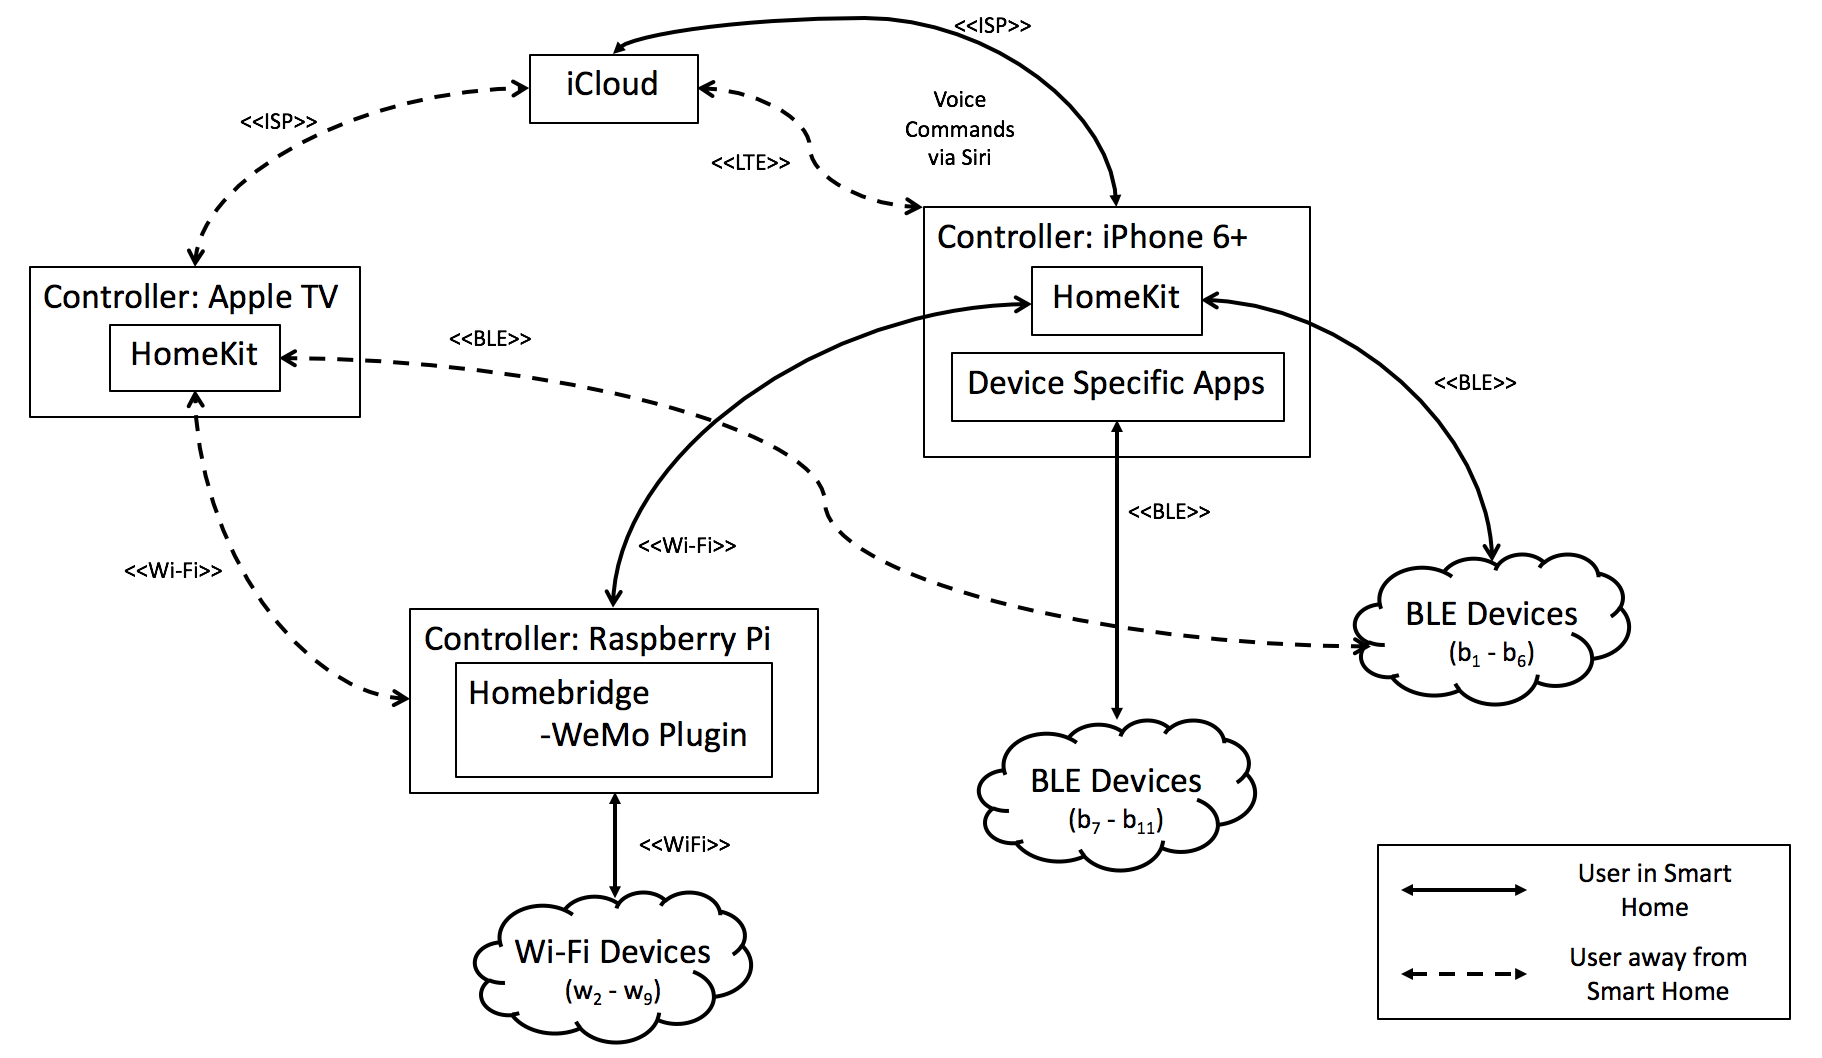
\includegraphics[width=\linewidth]{shaaDiagram}
			\caption{Diagram of SHAA components}
			\label{fig:ShaaDiagram}
		\end{center}
		\vspace{-0.2 in}
	\end{figure*}
}

\newcommand{\figCitiotDiagram}{
	\begin{figure*}[h!]
		\begin{center}
			\makebox[\textwidth][c]{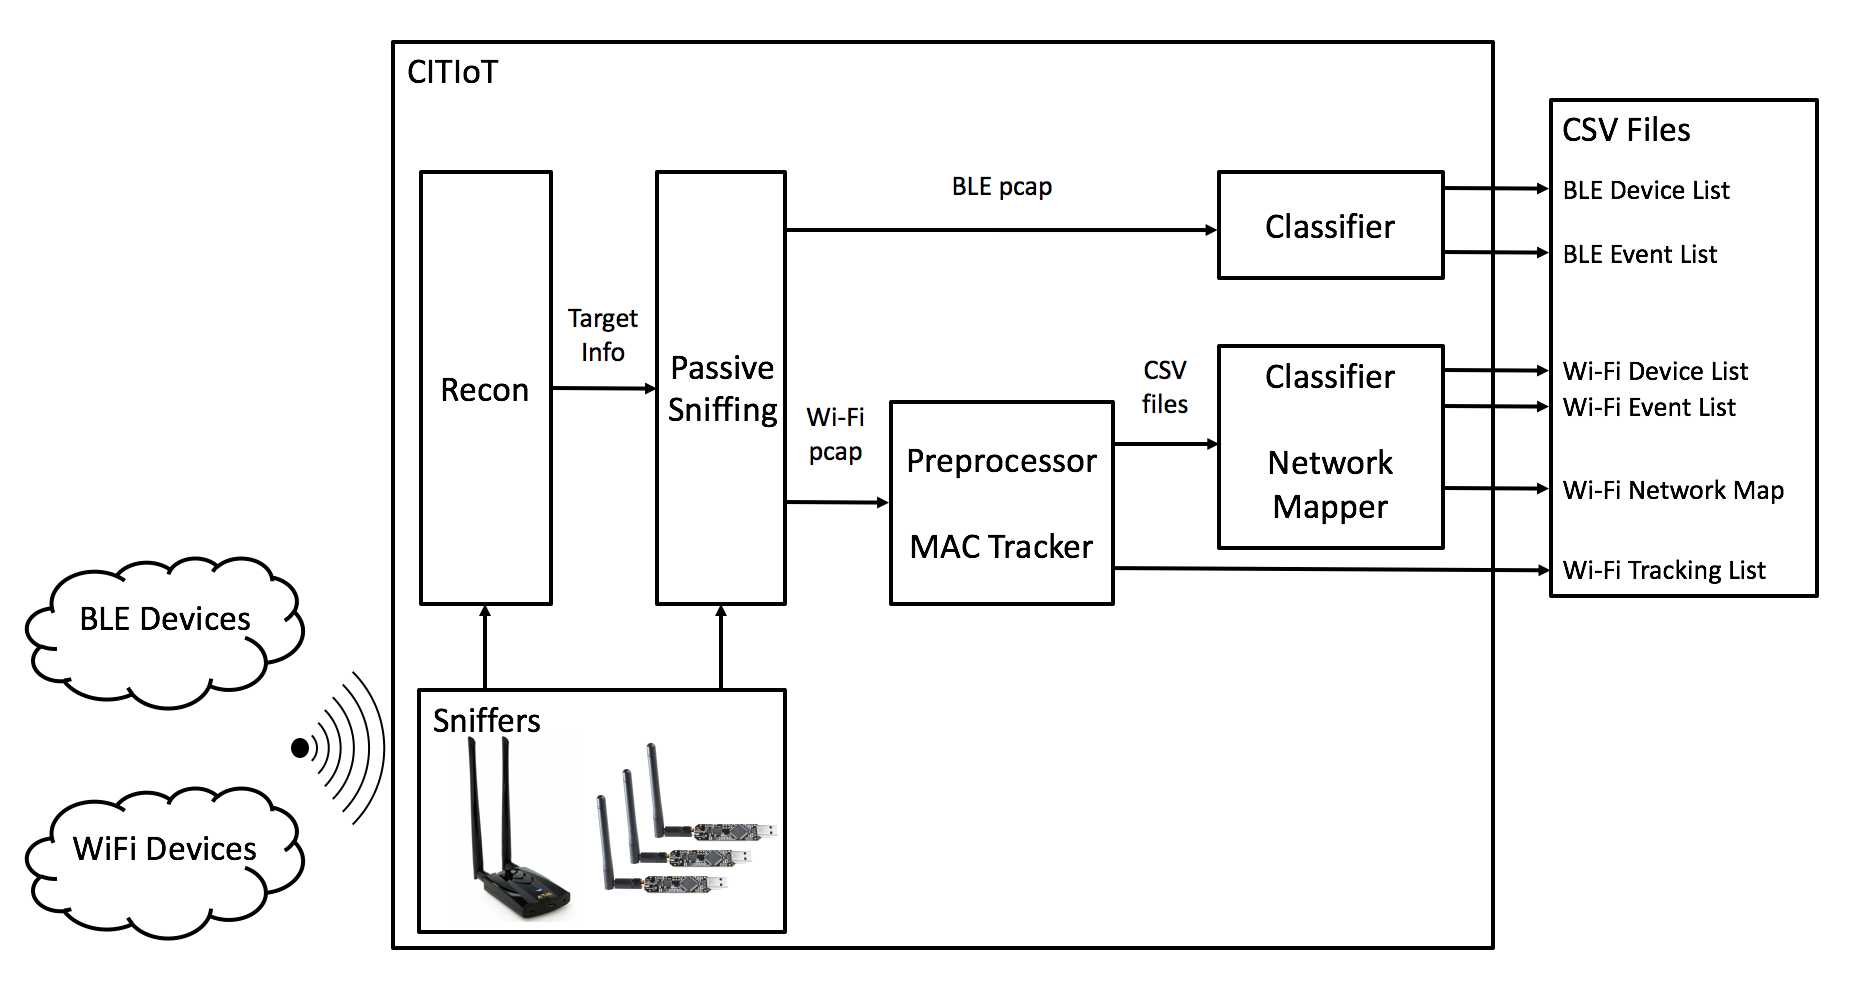
\includegraphics[width=\linewidth]{citiotDiagram}}
			\caption{Diagram of CITIoT tool components and interactions}
			\label{fig:CitiotDiagram}
		\end{center}
		\vspace{-0.2 in}
	\end{figure*}
}

\newcommand{\figReconScan}{
	\begin{figure*}[h!]
		\begin{center}
			\makebox[\textwidth][c]{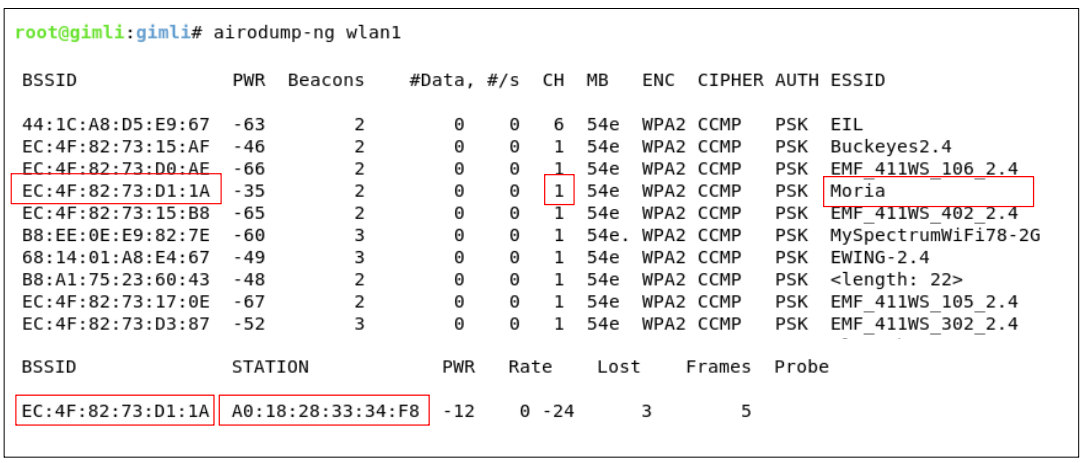
\includegraphics[width=\linewidth]{reconScan}}
			\caption{Command and results to accomplish a scan of Wi-Fi devices and associated \ac{AP}s}
			\label{fig:ReconScan}
		\end{center}
		\vspace{-0.2 in}
	\end{figure*}
}

\newcommand{\figScanDevices}{
	\begin{figure}[H]
		\begin{center}
			\makebox[\textwidth][c]{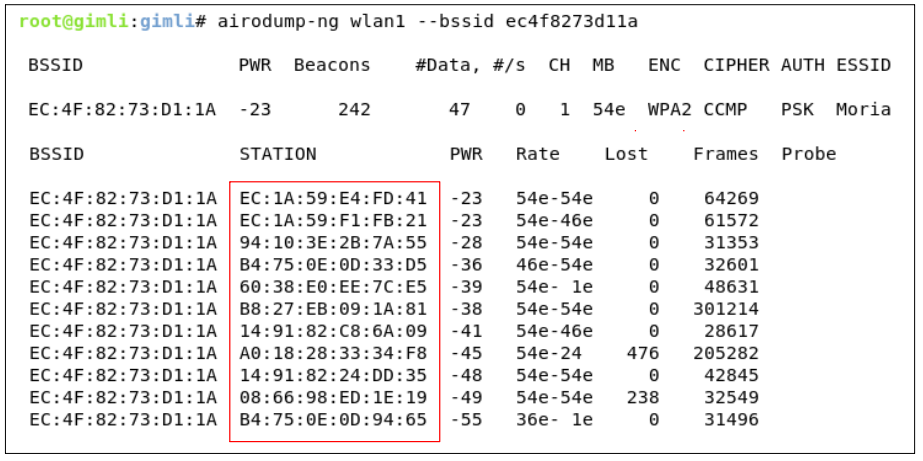
\includegraphics[width=\linewidth]{scanDevices}}
			\caption{Command and results to scan for devices connected to the target \ac{AP}}
			\label{fig:ScanDevices}
		\end{center}
		\vspace{-0.2 in}
	\end{figure}
}

\newcommand{\figOuiLookup}{
	\begin{figure}[H]
		\begin{center}
			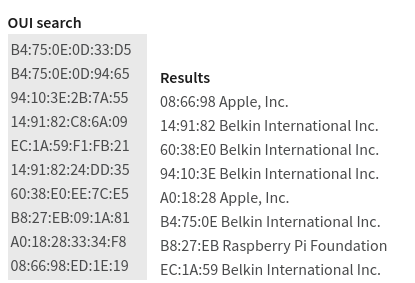
\includegraphics[width=3in]{ouiLookup}
			\caption{Wi-Fi MAC OUI search and results}
			\label{fig:OuiLookup}
		\end{center}
		\vspace{-0.2 in}
	\end{figure}
}

\newcommand{\figBleDeviceScan}{
	\begin{figure}[H]
		\begin{center}
			\makebox[\textwidth][c]{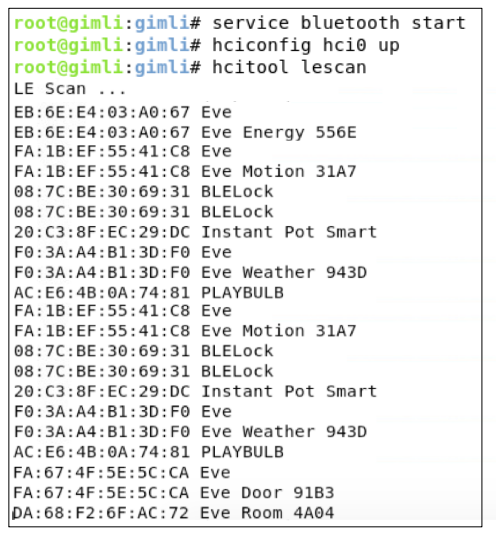
\includegraphics[width=3.5in]{bleDeviceScan}}
			\caption{Command and results to scan for \ac{BLE} devices within the smart home}
			\label{fig:BleDeviceScan}
		\end{center}
		\vspace{-0.2 in}
	\end{figure}
}

\newcommand{\figMonitorMode}{
	\begin{figure}[H]
		\begin{center}
			\makebox[\textwidth][c]{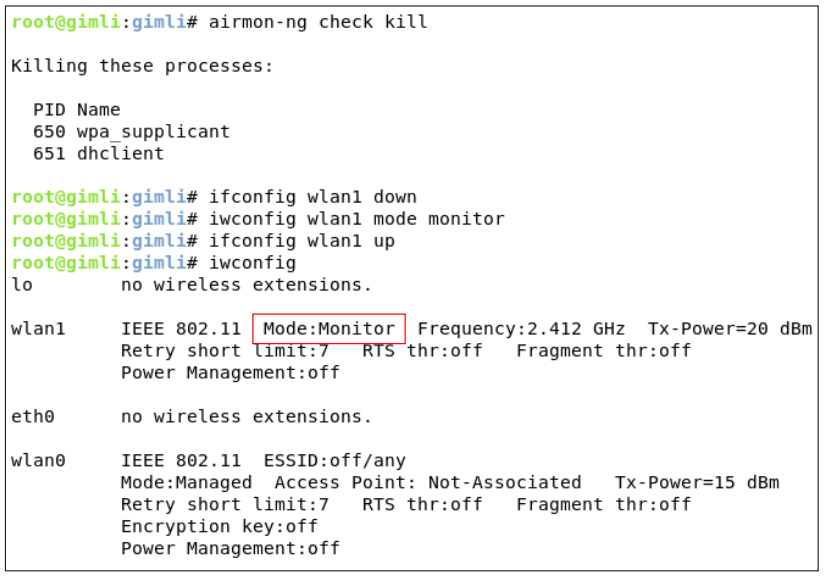
\includegraphics[width=\linewidth]{monitorMode}}
			\caption{Commands used to set Wi-Fi interface to monitor mode}
			\label{fig:MonitorMode}
		\end{center}
		\vspace{-0.2 in}
	\end{figure}
}

\newcommand{\figWifiCaptCmd}{
	\begin{figure}[H]
		\begin{center}
			\makebox[\textwidth][c]{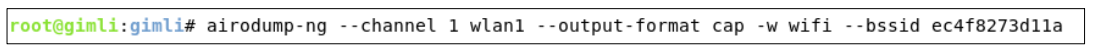
\includegraphics[height=.75cm]{wifiCaptCmd}}
			\caption{Command and options used to capture Wi-Fi traffic}
			\label{fig:WifiCaptCmd}
		\end{center}
		\vspace{-0.2 in}
	\end{figure}
}

\newcommand{\figBleCaptCmd}{
	\begin{figure}[H]
		\begin{center}
			\makebox[\textwidth][c]{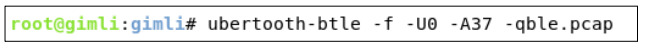
\includegraphics[height=.75cm]{bleCaptCmd}}
			\caption{Example command and options used to capture \ac{BLE} traffic}
			\label{fig:BleCaptCmd}
		\end{center}
		\vspace{-0.2 in}
	\end{figure}
}

\newcommand{\figCorruptTimePacket}{
	\begin{figure}[H]
		\begin{center}
			\makebox[\textwidth][c]{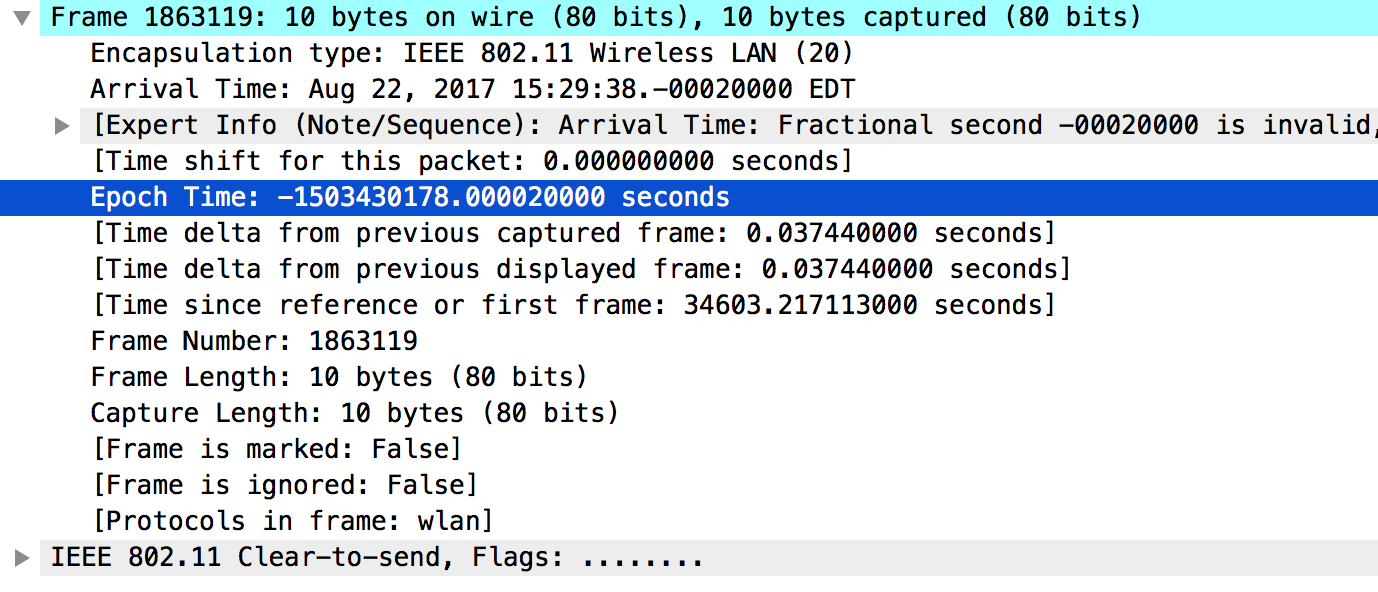
\includegraphics[width=\linewidth]{corruptTimePacket}}
			\caption{Encrypted packet used in \ac{MAC} tracker showing corrupted timestamp}
			\label{fig:CorruptTimePacket}
		\end{center}
		\vspace{-0.2 in}
	\end{figure}
}

\newcommand{\figWrongFrameNumber}{
	\begin{figure}[H]
		\begin{center}
			\makebox[\textwidth][c]{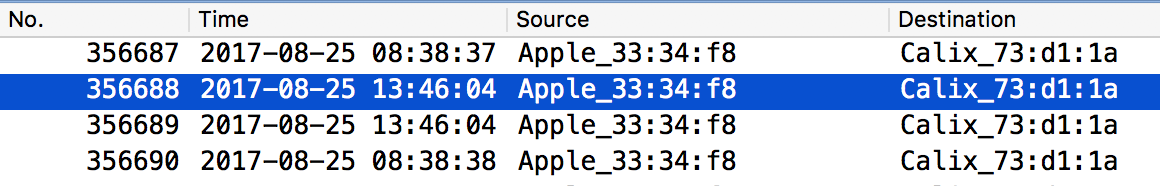
\includegraphics[width=\linewidth]{wrongFrameNumber}}
			\caption{Encrypted packets used in \ac{MAC} tracker showing sequential frame numbers but wrong times}
			\label{fig:WrongFrameNumber}
		\end{center}
		\vspace{-0.2 in}
	\end{figure}
}

\newcommand{\figTrainingToDevice}{
	\begin{figure}[H]
		\centering
		\begin{subfigure}{.485\textwidth}
			\centering
			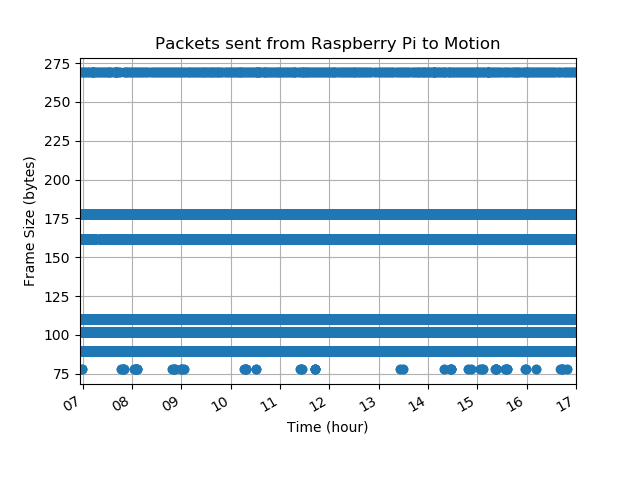
\includegraphics[width=\linewidth]{trngToMotion}
			\caption{}
		\end{subfigure}%
		\begin{subfigure}{.485\textwidth}
			\centering
			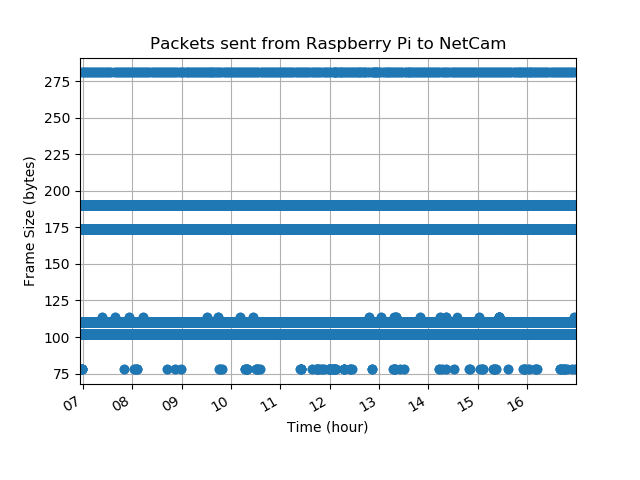
\includegraphics[width=\linewidth]{trngToNetcam}
			\caption{}
		\end{subfigure}
		\begin{subfigure}{.485\textwidth}
			\centering
			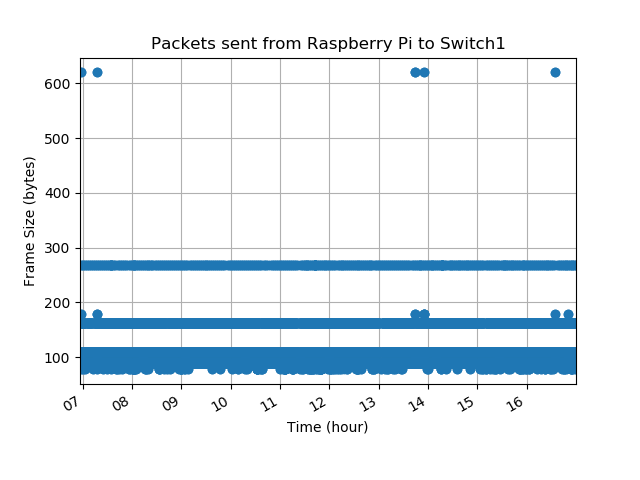
\includegraphics[width=\linewidth]{trngToSwitch1}
			\caption{}
		\end{subfigure}%
		\begin{subfigure}{.485\textwidth}
			\centering
			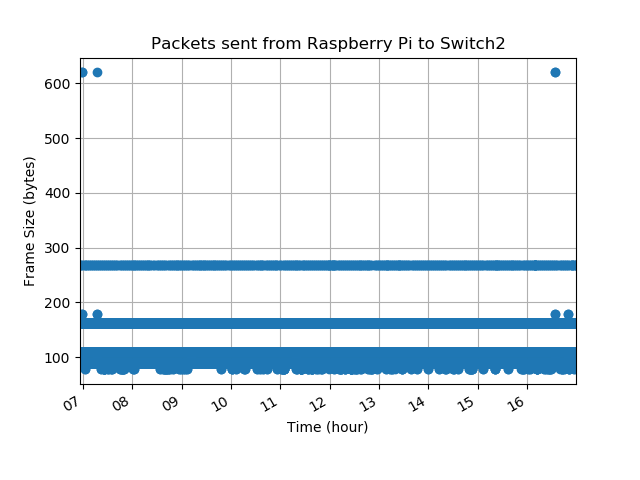
\includegraphics[width=\linewidth]{trngToSwitch2}
			\caption{}
		\end{subfigure}
		\begin{subfigure}{.485\textwidth}
			\centering
			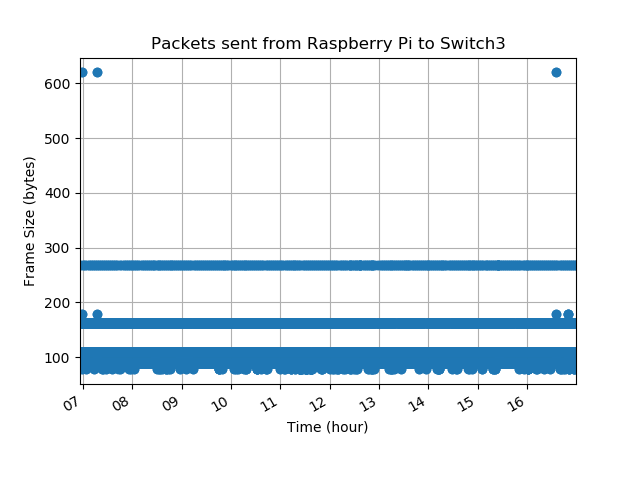
\includegraphics[width=\linewidth]{trngToSwitch3}
			\caption{}
		\end{subfigure}%
		\begin{subfigure}{.485\textwidth}
			\centering
			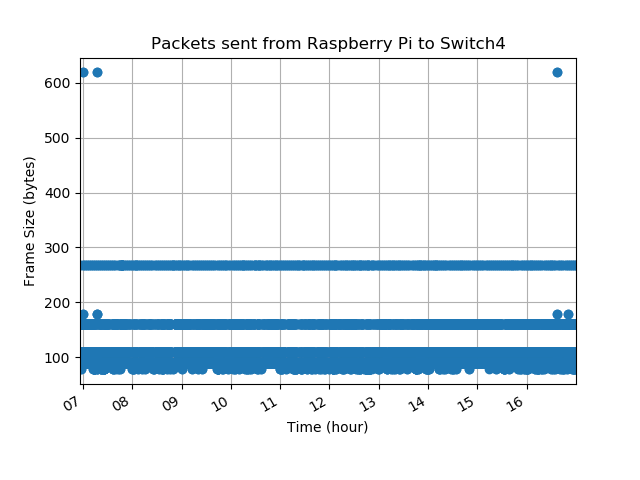
\includegraphics[width=\linewidth]{trngToSwitch4}
			\caption{}
		\end{subfigure}
		\begin{subfigure}{.485\textwidth}
			\centering
			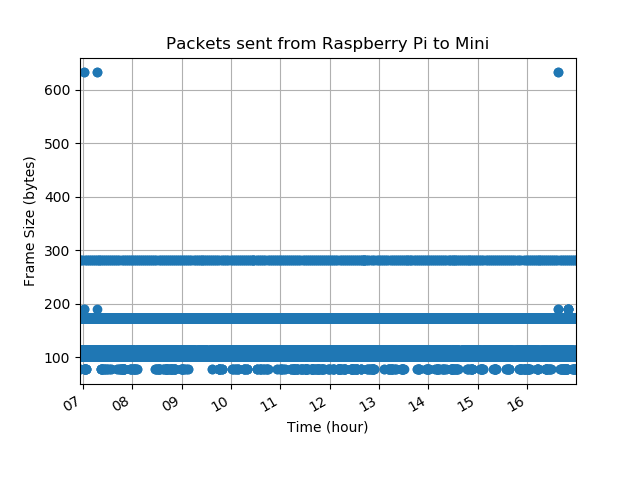
\includegraphics[width=\linewidth]{trngToMini}
			\caption{}
		\end{subfigure}%
		\begin{subfigure}{.485\textwidth}
			\centering
			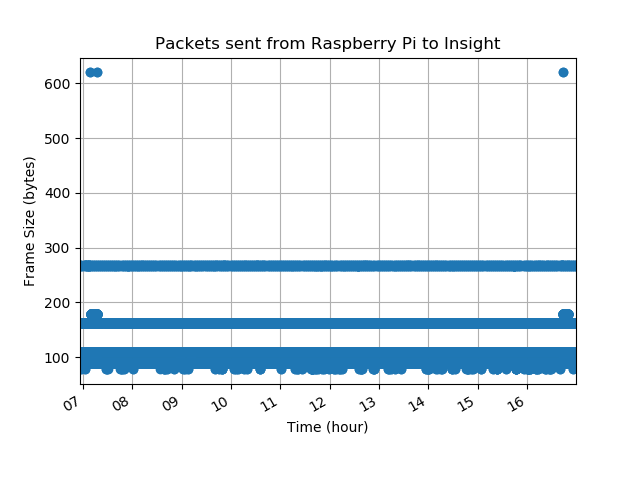
\includegraphics[width=\linewidth]{trngToInsight}
			\caption{}
		\end{subfigure}
		\caption{Training plots of packets sent from raspberry pi to device}
		\label{fig:TrainingToDevice}
	\end{figure}
}

\newcommand{\figTrainingFromDevice}{
	\begin{figure}[H]
		\centering
		\begin{subfigure}{.485\textwidth}
			\centering
			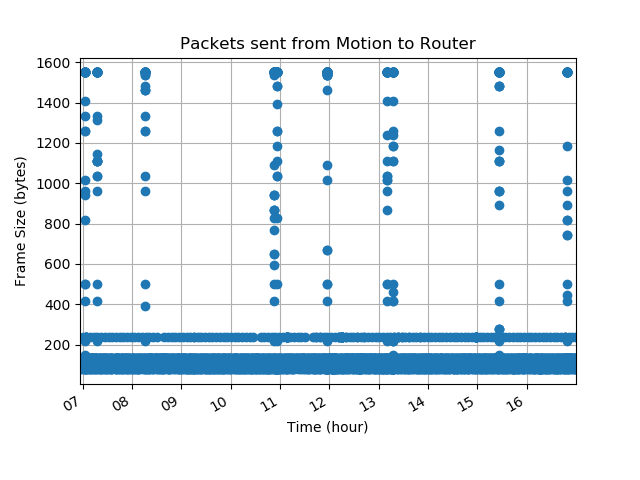
\includegraphics[width=\linewidth]{trngFromMotion}
			\caption{}
		\end{subfigure}%
		\begin{subfigure}{.485\textwidth}
			\centering
			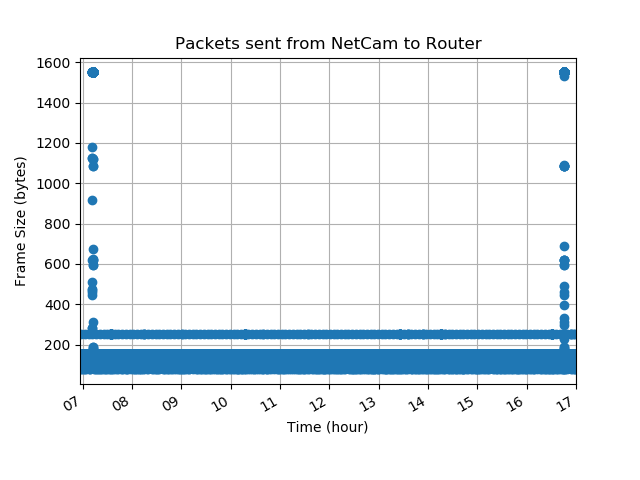
\includegraphics[width=\linewidth]{trngFromNetcam}
			\caption{}
		\end{subfigure}
		\begin{subfigure}{.485\textwidth}
			\centering
			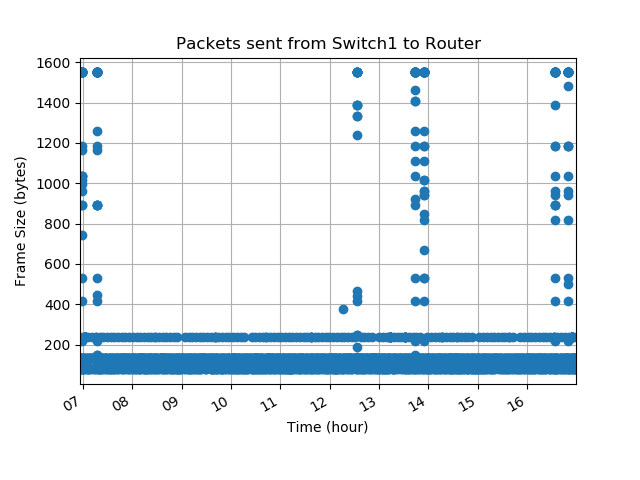
\includegraphics[width=\linewidth]{trngFromSwitch1}
			\caption{}
		\end{subfigure}%
		\begin{subfigure}{.485\textwidth}
			\centering
			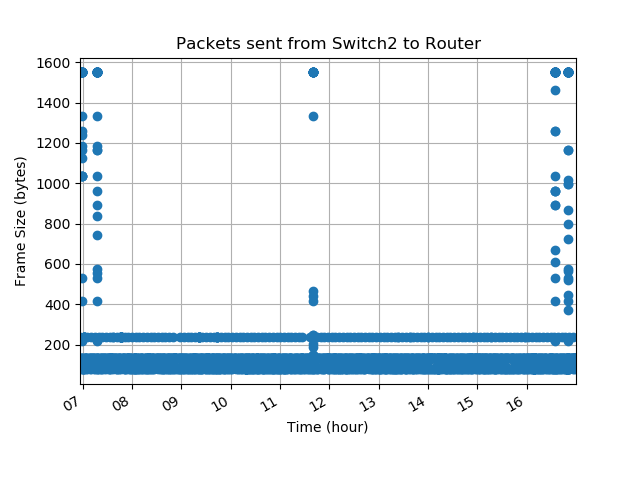
\includegraphics[width=\linewidth]{trngFromSwitch2}
			\caption{}
		\end{subfigure}
		\begin{subfigure}{.485\textwidth}
			\centering
			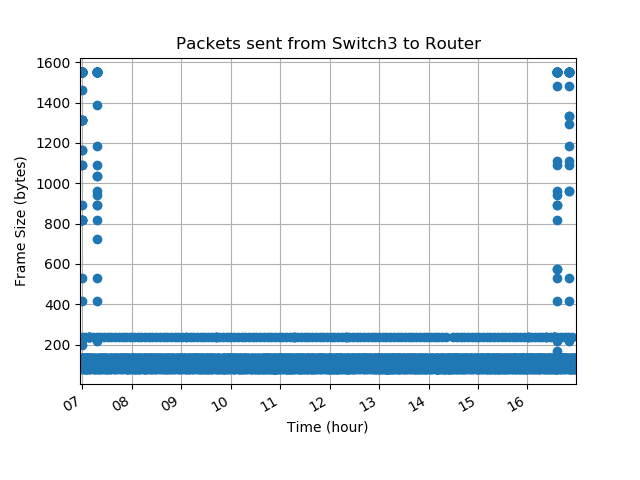
\includegraphics[width=\linewidth]{trngFromSwitch3}
			\caption{}
		\end{subfigure}%
		\begin{subfigure}{.485\textwidth}
			\centering
			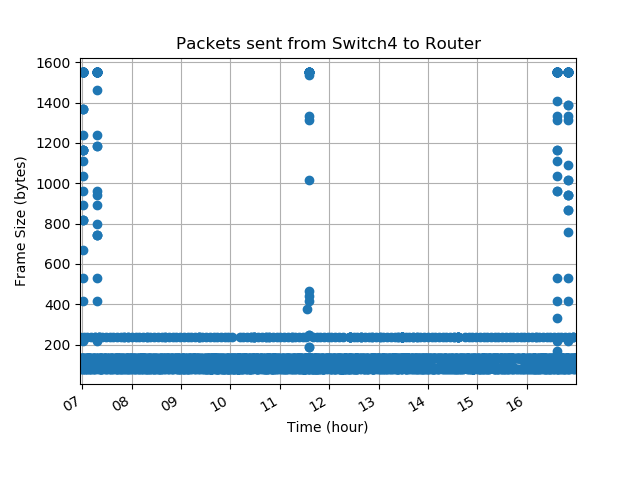
\includegraphics[width=\linewidth]{trngFromSwitch4}
			\caption{}
		\end{subfigure}
		\begin{subfigure}{.485\textwidth}
			\centering
			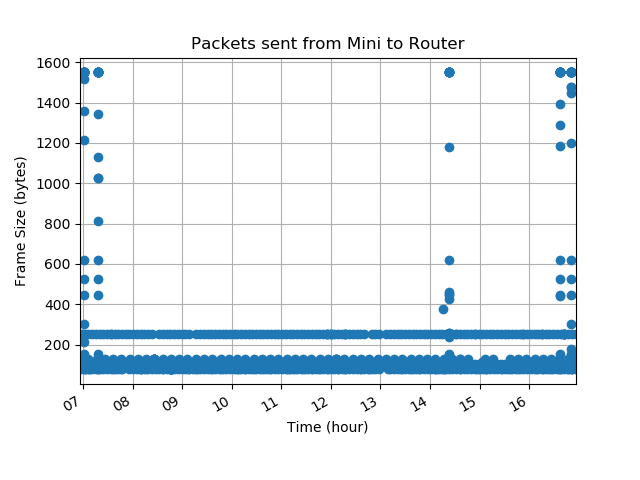
\includegraphics[width=\linewidth]{trngFromMini}
			\caption{}
		\end{subfigure}%
		\begin{subfigure}{.485\textwidth}
			\centering
			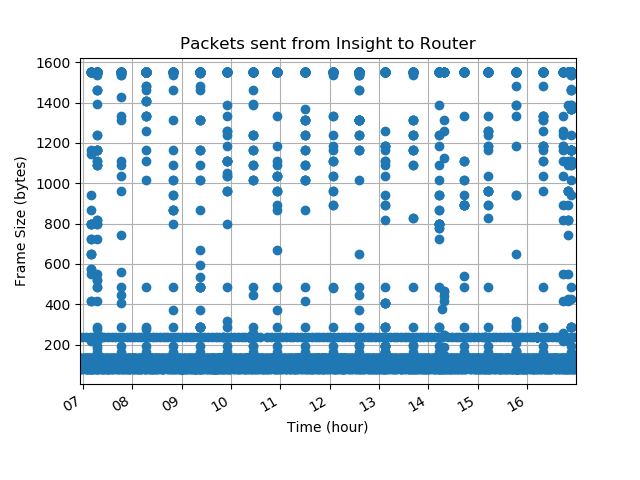
\includegraphics[width=\linewidth]{trngFromInsight}
			\caption{}
		\end{subfigure}
		\caption{Training plots of packets sent from device to the router}
		\label{fig:TrainingFromDevice}
	\end{figure}
}

\newcommand{\figClassificationToNetcam}{
	\begin{figure}[H]
		\begin{center}
			\makebox[\textwidth][c]{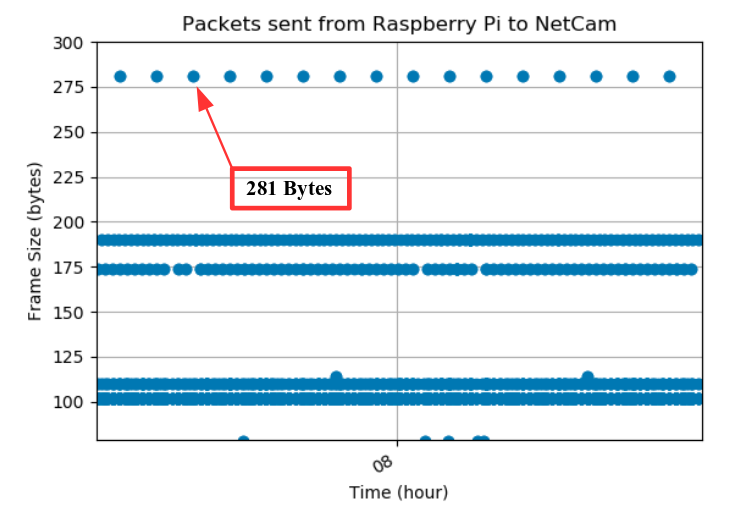
\includegraphics[width=5in]{classificationToNetcam}}
			\caption{Figure~\ref{fig:TrainingToDevice}(b) zoomed in on unique packet traffic used to classify camera devices}
			\label{fig:ClassificationToNetcam}
		\end{center}
		\vspace{-0.2 in}
	\end{figure}
}

\newcommand{\figClassificationToMotion}{
	\begin{figure}[H]
		\begin{center}
			\makebox[\textwidth][c]{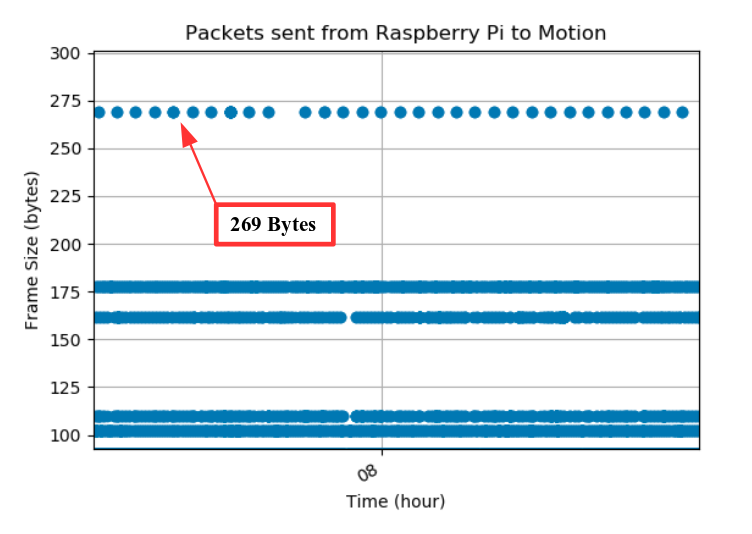
\includegraphics[width=5in]{classificationToMotion}}
			\caption{Figure~\ref{fig:TrainingToDevice}(a) zoomed in on unique packet traffic used to classify motion devices}
			\label{fig:ClassificationToMotion}
		\end{center}
		\vspace{-0.2 in}
	\end{figure}
}

\newcommand{\figClassificationToSwitch}{
	\begin{figure}[H]
		\begin{center}
			\makebox[\textwidth][c]{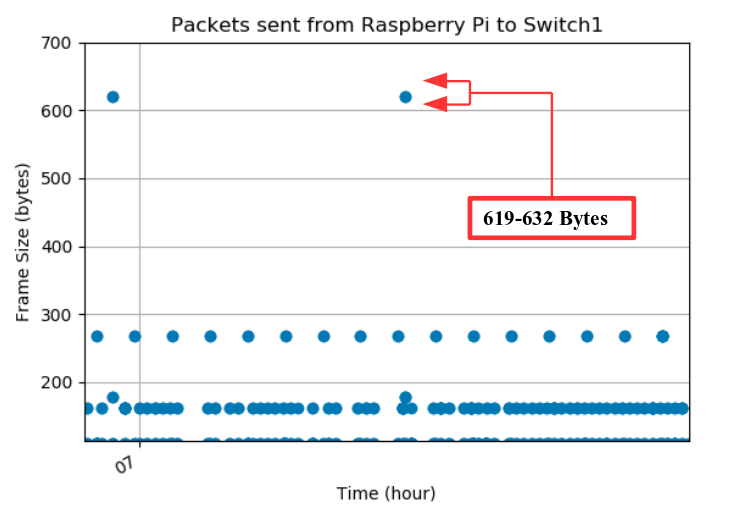
\includegraphics[width=5in]{classificationToSwitch}}
			\caption{Figure~\ref{fig:TrainingToDevice}(c) zoomed in on unique packet traffic used to classify outlet devices}
			\label{fig:ClassificationToSwitch}
		\end{center}
		\vspace{-0.2 in}
	\end{figure}
}

\newcommand{\figDeviceClassification}{
	\begin{figure}[H]
		\begin{center}
			\makebox[\textwidth][c]{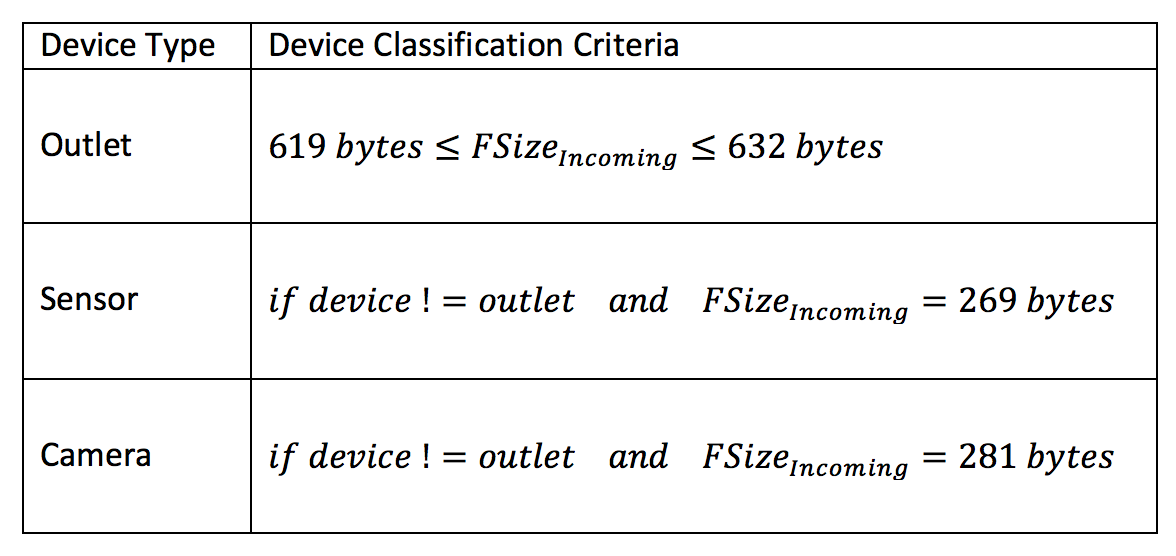
\includegraphics[height=2in]{deviceClassification}}
			\caption{Criteria used to classify devices}
			\label{fig:DeviceClassification}
		\end{center}
		\vspace{-0.2 in}
	\end{figure}
}

\newcommand{\figIdentificationToMini}{
	\begin{figure}[H]
		\begin{center}
			\makebox[\textwidth][c]{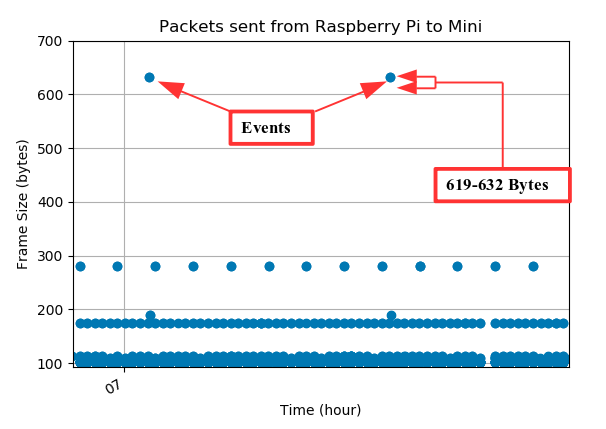
\includegraphics[width=5in]{identificationToMini}}
			\caption{Figure~\ref{fig:TrainingToDevice}(g) zoomed in on unique packet traffic used to identify outlet events}
			\label{fig:IdentificationToMini}
		\end{center}
		\vspace{-0.2 in}
	\end{figure}
}

\newcommand{\figIdentificationFromNetcam}{
	\begin{figure}[H]
		\begin{center}
			\makebox[\textwidth][c]{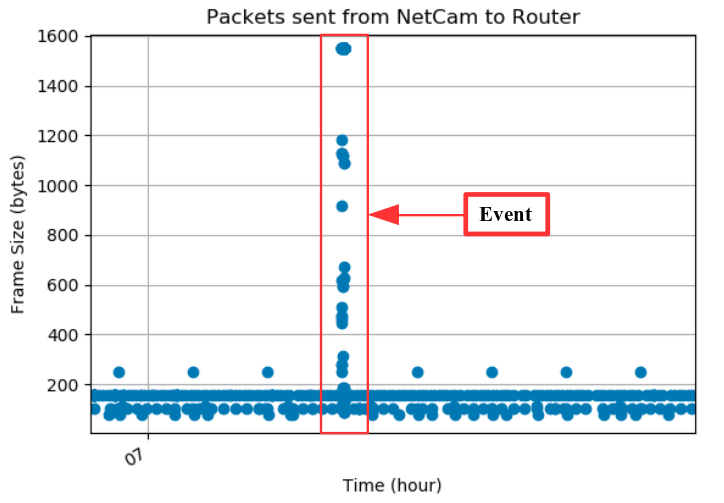
\includegraphics[width=5in]{identificationFromNetcam}}
			\caption{Figure~\ref{fig:TrainingFromDevice}(b) zoomed in on unique packet traffic used to identify camera events}
			\label{fig:IdentificationFromNetcam}
		\end{center}
		\vspace{-0.2 in}
	\end{figure}
}

\newcommand{\figIdentificationFromNetcamCum}{
	\begin{figure}[H]
		\begin{center}
			\makebox[\textwidth][c]{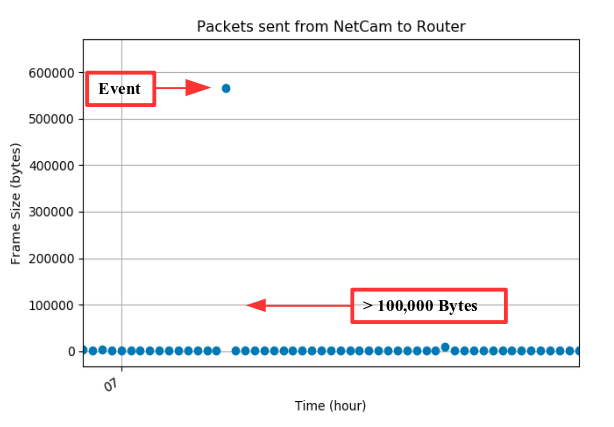
\includegraphics[width=5in]{identificationFromNetcamCum}}
			\caption{Figure~\ref{fig:TrainingFromDevice}(b) with one minute cumulative frame size zoomed in on unique packet traffic used to identify camera events}
			\label{fig:IdentificationFromNetcamCum}
		\end{center}
		\vspace{-0.2 in}
	\end{figure}
}

\newcommand{\figIdentificationFromMotion}{
	\begin{figure}[H]
		\begin{center}
			\makebox[\textwidth][c]{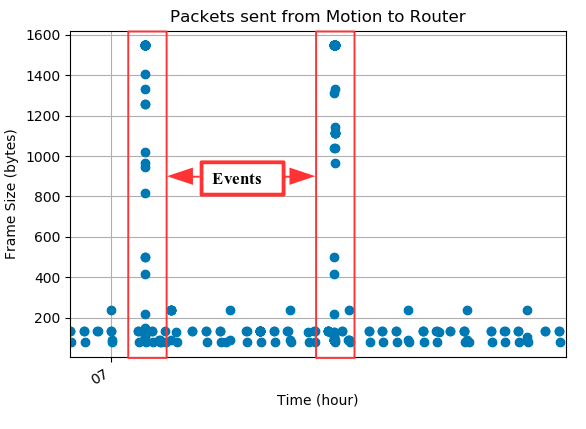
\includegraphics[width=5in]{identificationFromMotion}}
			\caption{Figure~\ref{fig:TrainingFromDevice}(a) zoomed in on unique packet traffic used to identify motion events}
			\label{fig:IdentificationFromMotion}
		\end{center}
		\vspace{-0.2 in}
	\end{figure}
}

\newcommand{\figIdentificationFromMotionCum}{
	\begin{figure}[H]
		\begin{center}
			\makebox[\textwidth][c]{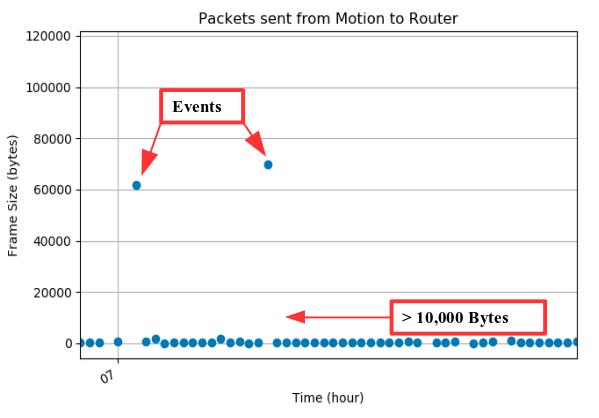
\includegraphics[width=5in]{identificationFromMotionCum}}
			\caption{Figure~\ref{fig:TrainingFromDevice}(a) with one minute cumulative frame size zoomed in on unique packet traffic used to identify motion events}
			\label{fig:IdentificationFromMotionCum}
		\end{center}
		\vspace{-0.2 in}
	\end{figure}
}

\newcommand{\figEventIdentification}{
	\begin{figure}[H]
		\begin{center}
			\makebox[\textwidth][c]{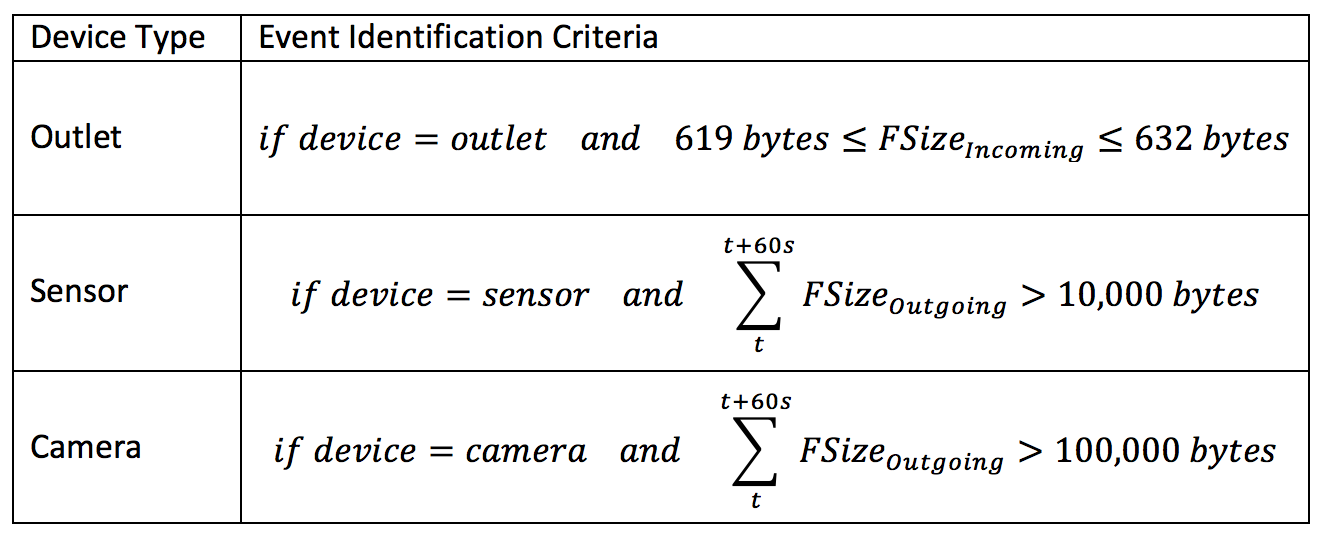
\includegraphics[height=2in]{eventIdentification}}
			\caption{Criteria used to identify events}
			\label{fig:EventIdentification}
		\end{center}
		\vspace{-0.2 in}
	\end{figure}
}

\newcommand{\figSubscribePacket}{
	\begin{figure}[H]
		\begin{center}
			\makebox[\textwidth][c]{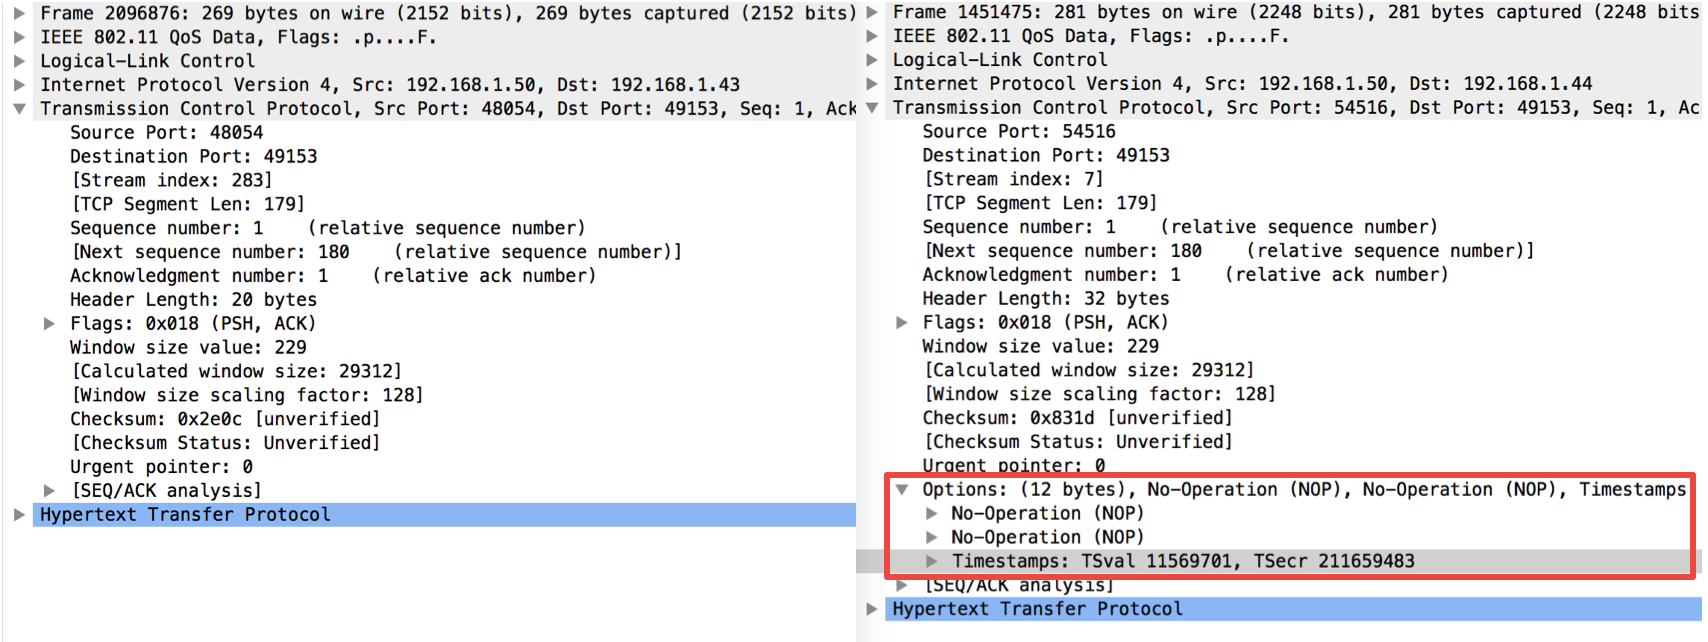
\includegraphics[width=\linewidth]{subscribePacket}}
			\caption{Decrypted \texttt{SUBSCRIBE} packets from Raspberry Pi to the NetCam and Motion devices depicting difference in frame length}
			\label{fig:SubscribePacket}
		\end{center}
		\vspace{-0.2 in}
	\end{figure}
}

\newcommand{\figPostPacket}{
	\begin{figure}[H]
		\begin{center}
			\makebox[\textwidth][c]{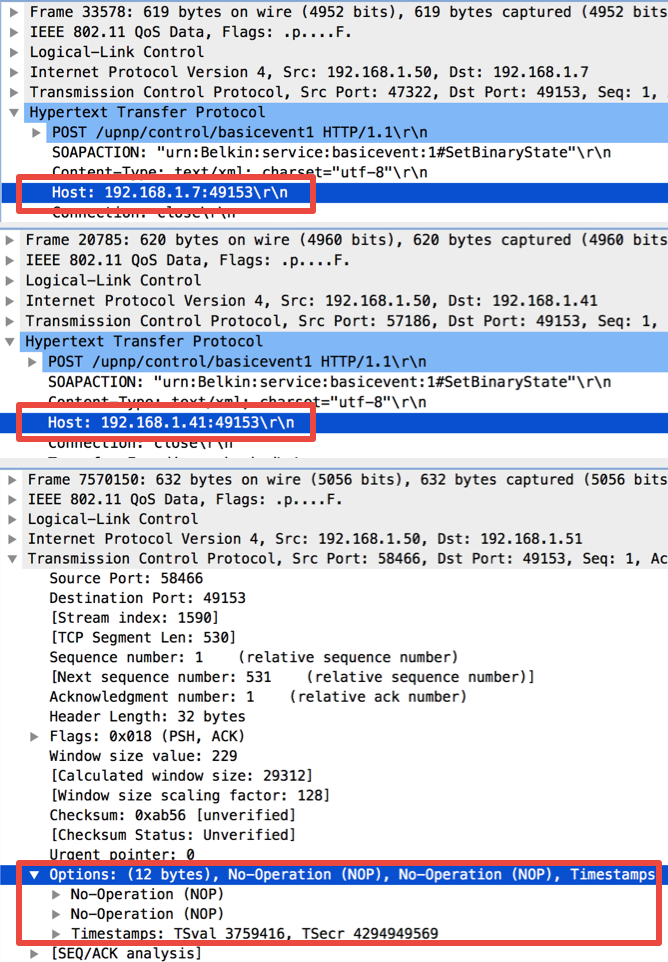
\includegraphics[width=.975\linewidth]{postPacket}}
			\caption{Decrypted \texttt{POST} packets from Raspberry Pi to the Switch4, Switch2, and Mini depicting differences in frame length}
			\label{fig:PostPacket}
		\end{center}
		\vspace{-0.2 in}
	\end{figure}
}

\newcommand{\figNetworkMap}{
	\begin{figure}[H]
		\begin{center}
			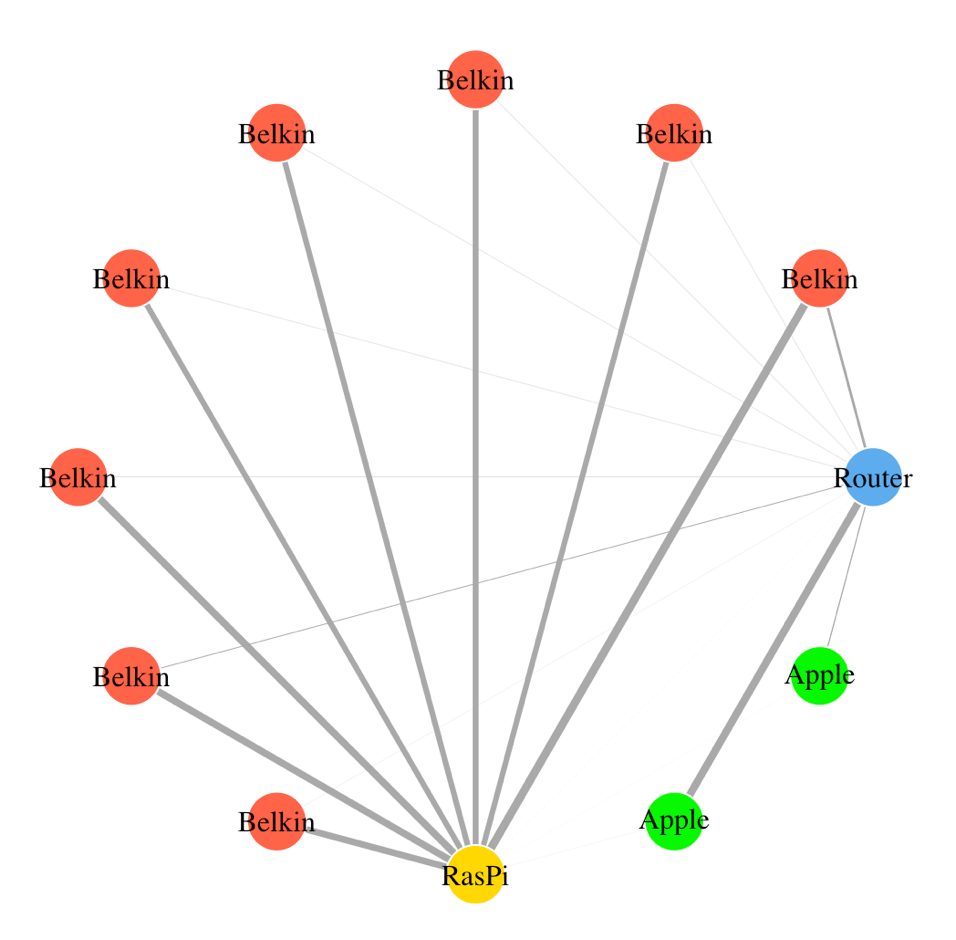
\includegraphics[width=5in]{networkMap}
			\caption{Network mapping of smart home architecture}
			\label{fig:NetworkMap}
		\end{center}
		\vspace{-0.2 in}
	\end{figure}
}

\newcommand{\figMiotlDiagram}{
	\begin{figure*}[h!]
		\begin{center}
			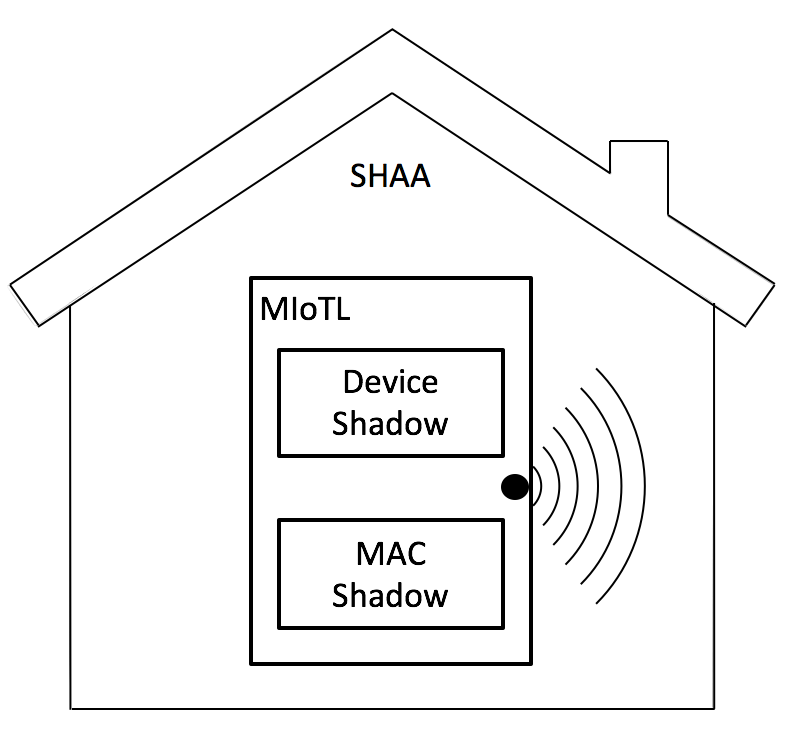
\includegraphics[width=3in]{miotlDiagram}
			\caption{Diagram of MIoTL tool components}
			\label{fig:MiotlDiagram}
		\end{center}
		\vspace{-0.2 in}
	\end{figure*}
}

\newcommand{\figSutCutDiagram}{
	\begin{figure*}[h!]
		\begin{center}
			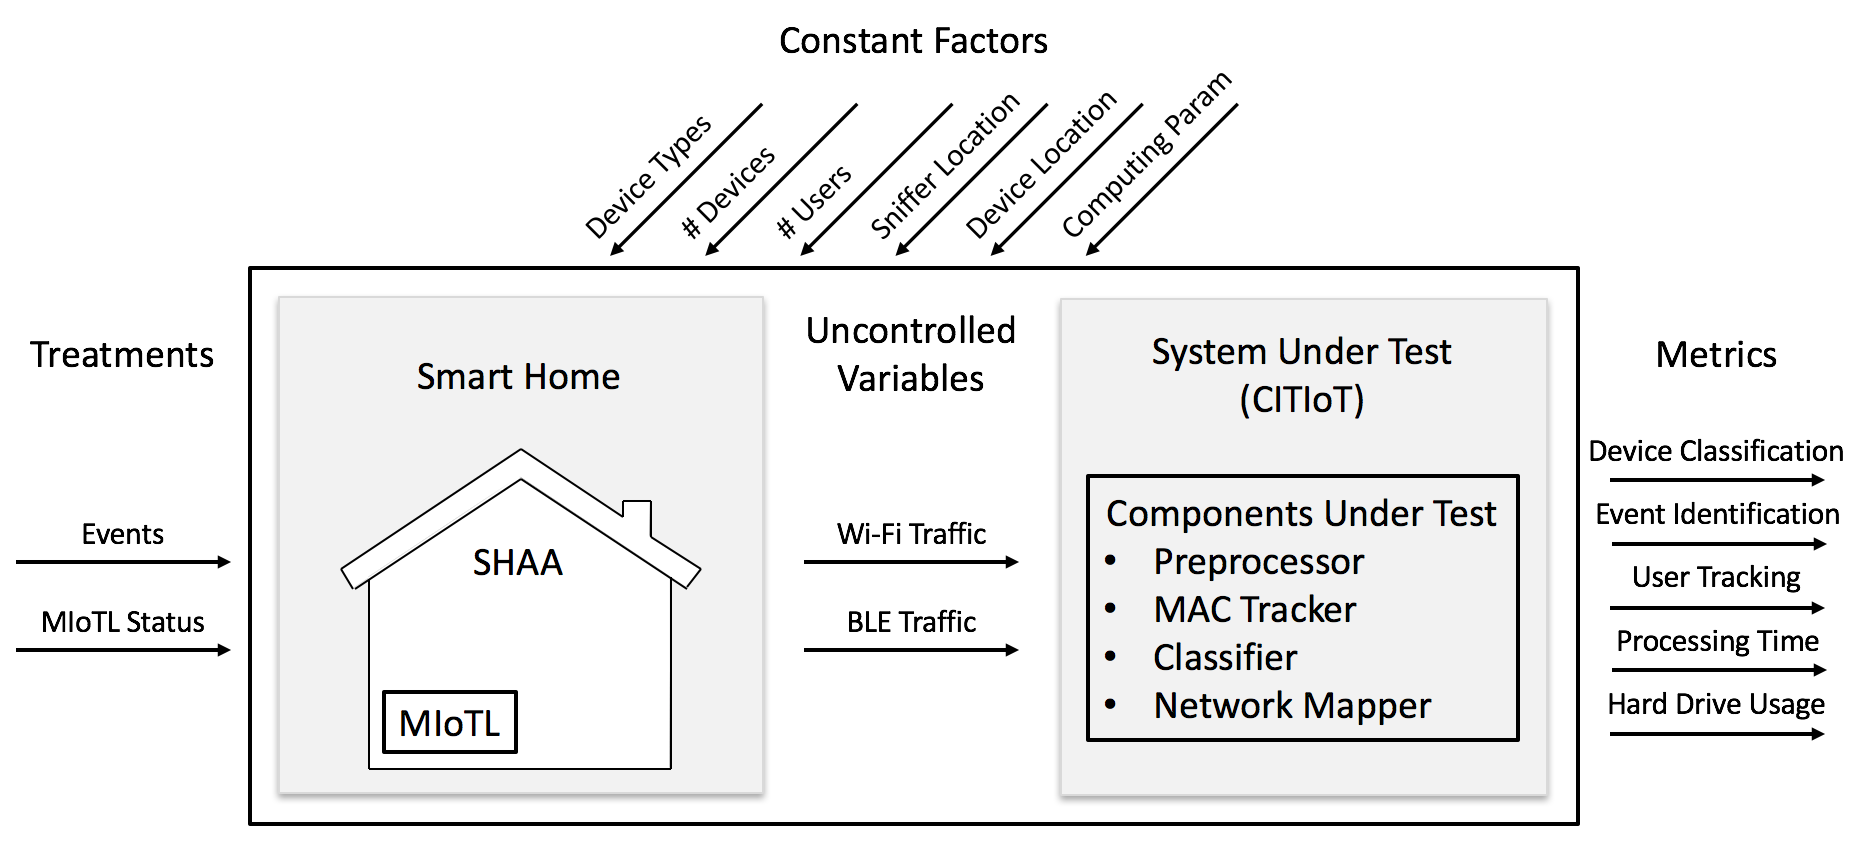
\includegraphics[width=\linewidth]{sutCutDiagram}
			\caption{System Under Test (SUT) and Component Under Test (CUT) diagram}
			\label{fig:SutCutDiagram}
		\end{center}
		\vspace{-0.2 in}
	\end{figure*}
}

\newcommand{\figShaaExperimentDiagram}{
	\begin{figure*}[h!]
		\begin{center}
			\includegraphics[width=\linewidth]{shaaExperimentDiagram}
			\caption{Approximate layout of devices within \ac{SHAA} for experimentation (not to scale)}
			\label{fig:ShaaExperimentDiagram}
		\end{center}
		\vspace{-0.2 in}
	\end{figure*}
}

\newcommand{\figSnifferExperimentSetup}{
	\begin{figure*}[h!]
		\begin{center}
			\includegraphics[width=\linewidth]{snifferExperimentSetup}
			\caption{Layout of sniffer antennae for experimentation}
			\label{fig:SnifferExperimentSetup}
		\end{center}
		\vspace{-0.2 in}
	\end{figure*}
}

\newcommand{\figDataCollectionFramework}{
	\begin{figure}[h!]
		\begin{center}
			\includegraphics[width=\linewidth, height = 5cm]{hostMachine}
			\caption{Data Collection Framework}
			\label{fig:DataCollectionFramework}
		\end{center}
		\vspace{-0.2 in}
	\end{figure}
}

\newcommand{\figSampleResults}{
\begin{figure}[H]
	\begin{center}
		\includegraphics[width=\linewidth]{sampleResults}
		\caption{Example graph comparing CITIoT events with actual events}
		\label{fig:SampleResults}
	\end{center}
	\vspace{-0.2 in}
\end{figure}
}

\newcommand{\figCitiot}{
	\begin{figure}[H]
		\begin{center}
			\makebox[\textwidth][c]{\includegraphics[width=5in]{citiot}}
			\caption{CITIoT Architecture}
			\label{fig:Citiot}
		\end{center}
		\vspace{-0.2 in}
	\end{figure}
}

\newcommand{\figReconScanning}{
	\begin{figure}[H]
		\begin{center}
			\makebox[\textwidth][c]{\includegraphics[width=5in]{reconScanning}}
			\caption{Scanning command along with output.}
			\label{fig:ReconScanning}
		\end{center}
		\vspace{-0.2 in}
	\end{figure}
}

\newcommand{\figNetworkMapping}{
	\begin{figure}[tbp]
		\begin{center}
			\includegraphics[width=3in, height=7cm]{networkMapping}
			\caption{Network mapping of smart home architecture; thicker lines mean stronger correlation between devices.}
			\label{fig:NetworkMapping}
		\end{center}
		\vspace{-0.2 in}
	\end{figure}
}

\newcommand{\figMethodologyOverview}{
	\begin{figure}[H]
		\begin{center}
			\makebox[\textwidth][c]{\includegraphics[width=6in]{methodologyOverview}}
			\caption{Overall scenario setup.}
			\label{fig:MethodologyOverview}
		\end{center}
		\vspace{-0.2 in}
	\end{figure}
}

\newcommand{\figDeviceId}{
	\begin{figure}[H]
	\centering
		\begin{minipage}{.5\textwidth}
			\centering
			\includegraphics[width=1\linewidth]{deviceIdOutlet}
			\caption{Outlet device.}
			\label{fig:DeviceIdOutlet}
		\end{minipage}%
		\begin{minipage}{.5\textwidth}
			\centering
			\includegraphics[width=1\linewidth]{deviceIdSensor}
			\caption{Sensor device.}
			\label{fig:DeviceIdSensor}
		\end{minipage}
		\begin{minipage}{.5\textwidth}
			\centering
			\includegraphics[width=1\linewidth]{deviceIdCamera}
			\caption{Camera device.}
			\label{fig:DeviceIdCamera}
		\end{minipage}
	\end{figure}
}


\newcommand{\figExamplePlotOne}{
	\begin{figure}[H]
		\begin{center}
			\makebox[\textwidth][c]{\includegraphics[width=4.5in]{examplePlot1}}
			\caption{Example Plot One: Event Identification}
			\label{fig:ExamplePlotOne}
		\end{center}
		\vspace{-0.2 in}
	\end{figure}
}

\newcommand{\figExamplePlotTwo}{
	\begin{figure}[H]
		\begin{center}
			\makebox[\textwidth][c]{\includegraphics[width=4.5in]{examplePlot2}}
			\caption{Example Plot Two: Time User is Home}
			\label{fig:ExamplePlotTwo}
		\end{center}
		\vspace{-0.2 in}
		\end{figure}
}

\newcommand{\figafitStyle}{\begin{figure}[tbp]
 \begin{center}
    \includegraphics[width=6in]{myFirstLaTeXafit}
     \caption{Recompile using afitThesis.sty, the AFIT
     thesis style file.}
     \label{fig:afitStyle}
 \end{center}
\end{figure}
}


\newcommand{\figtitlePage}{\begin{figure}[tbp]
 \begin{center}
    \includegraphics[width=6in]{titlePage}
     \caption{Enter student data in titlePage.tex to customize the
     document's first pages.}
     \label{fig:titlePage}
 \end{center}
\end{figure}
}

\newcommand{\figmyFlypage}{\begin{figure}[tbp]
 \begin{center}
    \includegraphics[width=6in]{myFlypage}
     \caption{Here we have compiled the first four page of a thesis.}
     \label{fig:myFlypage}
 \end{center}
\end{figure}
}

\newcommand{\figmyFirstAbstract}{\begin{figure}[tbp]
 \begin{center}
    \includegraphics[width=6in]{myFirstAbstract}
     \caption{Add an abstract to the front matter of your thesis.}
     \label{fig:myFirstAbstract}
 \end{center}
\end{figure}
}

\newcommand{\figmyFigures}{\begin{figure}[tbp]
 \begin{center}
    \includegraphics[width=5in]{myFigures}
     \caption{Consider defining all your figures in one file.}
     \label{fig:myFigures}
 \end{center}
\end{figure}
}


\newcommand{\figmyFirstFigures}{\begin{figure}[tbp]
 \begin{center}
    \includegraphics[width=6in]{myFirstFigures}
     \caption{Add figures in the main matter of your document; fill in
     the document around your graphics.}
     \label{fig:myFirstFigures}
 \end{center}
\end{figure}
}

\newcommand{\figmyFirstBibTeX}{\begin{figure}[tbp]
 \begin{center}
    \includegraphics[width=6in]{myFirstBibTeX}
     \caption{Add your bibliography.}
     \label{fig:myFirstBibTeX}
 \end{center}
\end{figure}
}




\newcommand{\tableWifiDevices}{
\begin{table}[H]
	\centering
	\caption{Wi-Fi Devices.}\label{tbl:WifiDevices}
	\makebox[\textwidth][c]{\begin{tabular} {| c | c | c | c | c | c |}
		\hline
		\thead{ID} & \thead{Manuf} & \thead{Device Type} & \thead{Device Name} &  \thead{MAC} & \thead{IP Address} \\ 
		\hline
		w$_1 $ & Calix & Wireless Router & Moria & EC:4F:82:73:D1:1A & - \\
		\hline
		w$_2 $ & Belkin & Camera & NetCam & EC:1A:59:E4:FD:41 & 192.168.1.44 \\
		\hline
		w$_3 $ & Belkin & Outlet & Switch1 & B4:75:0E:0D:33:D5 & 192.168.1.40 \\
		\hline
		w$_4 $ & Belkin & Outlet & Switch2 & B4:75:0E:0D:94:65 & 192.168.1.41 \\
		\hline
		w$_5 $ & Belkin & Outlet & Switch3 & 94:10:3E:2B:7A:55 & 192.168.1.42 \\
		\hline
		w$_6 $ & Belkin & Outlet & Switch4 & 14:91:82:C8:6A:09 & 192.168.1.7 \\
		\hline
		w$_7 $ & Belkin & Motion Sensor & Motion & EC:1A:59:F1:FB:21 & 192.168.1.43 \\
		\hline
		w$_8 $ & Belkin & Outlet & Insight & 14:91:82:24:DD:35 & 192.168.1.47 \\
		\hline
		w$_9 $ & WeMo & Outlet & Mini & 60:38:E0:EE:7C:E5 & 192.168.1.51 \\
		\hline
		w$_{10} $ & Raspberry Pi 3B & Computer & Pi & B8:27:EB:09:1A:81 & 12.168.1.50 \\
		\hline
		w$_{11} $ & Apple & iPhone 6+ & Steves-phone & A0:18:28:33:34:F8 & 192.168.1.4 \\
		\hline
		w$_{12} $ & Apple & TV 2 & Apple-TV & 08:66:98:ED:1E:19 & 192.168.1.54 \\
		\hline
	\end{tabular}}
\end{table}
}

\newcommand{\tableWifiDeviceShort}{
	\begin{table}[tbp]
		\centering
		\caption{Wi-Fi Devices.}\label{tbl:WifiDevicesShort}
			\begin{tabular} {| c | c | c | c |}
				\hline
				\thead{ID} & \thead{Manuf} & \thead{Device Type} & \thead{Device Name} \\ 
				\hline
				w$_1 $ & Calix & Wireless Router & Prancing Pony  \\
				\hline
				w$_{2-5} $ & Belkin & Outlet & Switch1-4 \\
				\hline
				w$_6 $ & WeMo & Outlet & Mini  \\
				\hline
				w$_7 $ & Belkin & Outlet & Insight  \\
				\hline
				w$_8 $ & Belkin & Motion Sensor & Motion \\
				\hline
				w$_9 $ & Belkin & Camera & NetCam  \\
				\hline
				w$_{10} $ & Raspberry Pi 3B & Computer & Pi \\
				\hline
				w$_{11} $ & Apple & iPhone 6+ & Steves-phone  \\
				\hline
				w$_{12} $ & Apple & TV 2 & Apple-TV \\
				\hline
			\end{tabular}
	\end{table}
}

\newcommand{\tableBtleDevicesShort}{
	\begin{table}[tbp]
		\centering
		\caption{BLE Devices.}\label{tbl:BtleDevicesShort}
\begin{tabular}{|c|c|c|c|}
	\hline
	\thead{ID} & \thead{Manuf} & \thead{Device Type} & \thead{Device Name} \\
	\hline
	b$ _1 $ & Elgato & Indoor Temperature & Eve Room \\
	\hline
	b$ _2 $ & Elgato & Outdoor Temperature & Eve Weather \\
	\hline
	b$ _3 $ & Elgato & Motion Sensor & Eve Motion \\
	\hline
	b$ _4 $ & Elgato & Outlet & Eve Energy \\
	\hline
	b$ _5 $ & Elgato & Door Sensor & Eve Door \\
	\hline
	b$ _6 $ & Instant Pot & Smart Cooker & Instant Pot \\
	\hline
	b$ _7 $ & MPow & Lightbulb & Playbulb \\
	\hline
	b$ _8 $ & ZKTeco & Lock & BioLock \\
	\hline
	b$ _{9} $ & BitLock & Lock & Bike lock \\
	\hline
	b$ _{10} $ & SafeTech & Gunsafe & Gunsafe \\
	\hline
	b$ _{11} $ & Apple & iPhone 6+ & Steves-phone \\
	\hline
	b$ _{12} $ & Apple & TV 2 & Apple TV \\
	\hline
\end{tabular}
\end{table}
}

\newcommand{\tableDeviceClassifier}{
	\begin{table*}[tbp]
		\centering
		\caption{Classifier Criterion.}\label{tbl:DeviceClassifier}
		\begin{tabular} {| c | c | c |}
			\hline
			\thead{Device Type} & \thead{Device Classification} & \begin{tabular}{@{}c@{}}\thead{Event Identification} \\ (Relies on Device Classification)\end{tabular} \\
			\hline
			Outlet & $FSize_{in} > 650\ bytes$ & $1,000 > FSize_{in} > 600\ bytes$ \\
			\hline
			Sensor & $device\ != outlet\ and\ all\ FSize_{in} < 275\ bytes$ & $100,000>\sum\limits_{t}^{t+1}FSize_{out}>10,000\ bytes$\\
			\hline
			Camera & $device\ != outlet\ and\ 275 < FSize_{in} < 300\ bytes$ & $\sum\limits_{t}^{t+1}FSize_{out}>100,000\ bytes$\\
			\hline
		\end{tabular}
	\end{table*}
}

\newcommand{\tableBtleDevices}{
\begin{table}[H]
	\centering
	\caption{BLE Devices.}\label{tbl:BtleDevices}
	\makebox[\textwidth][c]{\begin{tabular}{| c | c|c|c|}
		\hline
		\thead{ID} & \thead{Manuf} & \thead{Device Type} & \thead{Device Name} \\
		\hline
		b$ _1 $ & Elgato & Indoor Temperature & Eve Room \\
		\hline
		b$ _2 $ & Elgato & Outdoor Temperature & Eve Weather \\
		\hline
		b$ _3 $ & Elgato & Motion Sensor & Eve Motion \\
		\hline
		b$ _4 $ & Elgato & Outlet & Eve Energy \\
		\hline
		b$ _5 $ & Elgato & Switch & Eve Light \\
		\hline
		b$ _6 $ & Elgato & Door Sensor & Eve Door \\
		\hline
		b$ _7 $ & Instant Pot & Smartcooker & Instant Pot \\
		\hline
		b$ _8 $ & MPow & Lightbulb & Playbulb \\
		\hline
		b$ _9 $ & ZKTeco & Lock & BioLock \\
		\hline
		b$ _{10} $ & BitLock & Lock & Bike lock \\
		\hline
		b$ _{11} $ & SafeTech & Gunsafe & Gunsafe \\
		\hline
		b$ _{12} $ & Apple & iPhone 6+ & Steves-phone \\
		\hline
		b$ _{13} $ & Apple & TV 2 & Apple TV \\
		\hline
	\end{tabular}}
\end{table}
}

\newcommand{\tablePerformanceMetrics}{
	\begin{table}[H]
		\centering
		\caption{Performance Metrics}
		\makebox[\textwidth][c]{\begin{tabular}{|c|c|c|c|}
			\hline
			\thead{Metric} & \thead{Units} & \thead{Accepted Range} & \thead{Expected Value} \\
			\hline
			DCSR (Device Classification Success Rate) & \% & 0 to 100 & $>$ 75\% \\
			\hline
			EISR (Event Identification Success Rate) & \% & 0 to 100 & $>$ 75\% \\
			\hline
			EIFP (Event Identification False Positives) & \% & 0 to 100 & $>$ 75\% \\
			\hline
			EIFN (Event Identification False Negatives) & \% & 0 to 100 & $>$ 75\% \\
			\hline
			ULSR (User Location Success Rate) & \% & 0 to 100 & $>$ 75\% \\
			\hline
			CT (Completion Time) & minutes & 0 to $\infty$ & $<$ 120 minutes \\
			\hline
			HDU (Hard Drive Usage) & bytes & 0 to $\infty$ & $<$ 20 GB \\
			\hline
		\end{tabular}}
		\label{tbl:PerformanceMetrics}
	\end{table}
}

\newcommand{\tableEvents}{
	\begin{table}[h!]
		\centering
		\caption{Experiment Events}\label{tbl:Events}
		\begin{tabular}{|c|c|c|c|}
			\hline
			\ & \thead{Device Name} & \thead{Action} & \thead{Protocol} \\
			\hline
			1 & Bike Lock & Unlock & BLE \\
			\hline
			2 & BioLock & Unlock & BLE \\
			\hline
			3 & Instant Pot & Turn on & BLE \\
			\hline
			4 & Instant Pot & Turn off & BLE \\
			\hline
			5 & Gunsafe  & Open & BLE \\
			\hline
			6 & Gunsafe  & Close & BLE \\
			\hline
			7 & Eve Room & Get temperature in living room & BLE \\
			\hline
			8 & Eve Weather & Get temperature on patio & BLE \\
			\hline
			9 & Eve Door & Open & BLE \\
			\hline
			10 & Eve Door & Close & BLE \\
			\hline
			11 & Eve Energy & Turn on & BLE \\
			\hline
			12 & Eve Energy & Turn off & BLE \\
			\hline
			13 & Eve Motion & Activate motion sensor & BLE \\
			\hline
			14 & Playbulb & Turn on & BLE \\
			\hline
			15 & Playbulb & Turn off & BLE \\
			\hline
			16 & Switch1 & Turn on & Wi-Fi \\
			\hline
			17 & Switch1 & Turn off & Wi-Fi \\
			\hline
			18 & Switch2 & Turn on & Wi-Fi \\
			\hline
			19 & Switch2 & Turn off & Wi-Fi \\
			\hline
			20 & Switch3 & Turn on & Wi-Fi \\
			\hline
			21 & Switch3 & Turn off & Wi-Fi \\
			\hline
			22 & Switch4 & Turn on & Wi-Fi \\
			\hline
			23 & Switch4 & Turn off & Wi-Fi \\
			\hline
			24 & Mini & Turn on & Wi-Fi \\
			\hline
			25 & Mini & Turn off & Wi-Fi \\
			\hline
			26 & Insight & Turn on & Wi-Fi \\
			\hline
			27 & Insight & Turn off & Wi-Fi \\
			\hline
			28 & NetCam & Activate motion & Wi-Fi \\
			\hline
			29 & Motion & Activate motion sensor & Wi-Fi \\
			\hline
			30 & Steves-phone & Leave house & Wi-Fi and BLE \\
			\hline
			31 & Steves-phone & Arrive House & Wi-Fi and BLE \\
			\hline
		\end{tabular}
	\end{table}
}

\newcommand{\tableTreatments}{
	\begin{table}[h!]
		\centering
		\caption{Experiment Treatments}
		\begin{tabular}{|c|c|c|}
			\hline
			\thead{Trial} \# & \thead{Events Administered} & \thead{MIoTL Status} \\
			\hline
			1-5 & 1-31 & Off \\
			\hline
			6 & 16-31 & On \\
			\hline
		\end{tabular}
		\label{tbl:Treatments}
	\end{table}
}

\newcommand{\tableTools}{
\begin{table}[H]
	\centering
	\caption{Wi-Fi and \ac{BLE} tools used throughout this work.}
	\label{tbl:Tools}
	\makebox[\textwidth][c]{\begin{tabular}{|c|c|p{8cm}|}
		\hline
		\textbf{Tool Name} & \textbf{Version}     & \textbf{Description} \\ 
		\hline
		Ubertooth One      & Firmware: 2017-03R2  & Bluetooth sniffer with open-source firmware and hardware \cite{Ubertooth} \\
		\hline
		BlueZ              & 5.43                 & Linux Bluetooth stack with utilities to scan for \ac{BLE} devices and transmit packets \cite{Bluez}\\
		\hline
		Plugable USB	   & 2.0				  & Commercial Broadcom BCM20702-based Bluetooth adapter to communicate with Bluetooth Devices \\
		\hline
		Alfa Card		   & AWUS036ACH			  & 802.11ac Wireless Adapter\\
		\hline
		Airodump-ng		   & Aircrack-ng 1.2	  & Wi-Fi network security tool to capture raw 802.11 frames\\
		\hline
		Python			   & 2.7.10				  & Programming language used in scripting\\
		\hline
		Pyshark			   & 0.3.7.8			  & Python wrapper allowing python packet parsing with wireshark dissectors \cite{pyshark}\\
		\hline
		Scapy			   & 2.3.3				  & Interactive packet manipulation tool used to send or receive 802.11 packets \cite{scapy}\\
		\hline
	\end{tabular}}
\end{table}
}

\newcommand{\tableBleResults}{
	\begin{table}[tbp]
		\centering
		\caption{Summary of \ac{BLE} Results.}
		\label{tbl:BleResults}
		\begin{tabular}{|c|c|c|c|c|}
			\hline
			\textbf{Date} & \textbf{True Pos} & \textbf{False Neg} & \textbf{False Pos} & \textbf{\# Events} \\ 
			\hline
			Day 1 & No Data & No Data & No Data & No Data \\
			\hline
			Day 2 & 37 & 5 & 5 & 42\\
			\hline
			Day 3 & 40 & 1 & 3 & 41\\
			\hline
			Day 4 & 36 & 0 & 9 & 36\\
			\hline
			Day 5 & 31 & 2 & 4 & 33\\
			\hline
			\hline
			Average & 36 & 2 & 5.25 & 38\\
			\hline
		\end{tabular}
	\end{table}
}

\newcommand{\tableWifiResults}{
	\begin{table}[tbp]
		\centering
		\caption{Summary of Wi-Fi Results.}
		\label{tbl:WifiResults}
		\begin{tabular}{|c|c|c|c|c|}
			\hline
			\textbf{Date} & \textbf{True Pos} & \textbf{False Neg} & \textbf{False Pos} & \textbf{\# Events} \\ 
			\hline
			Day 1 & 31 & 0 & 0 & 31 \\
			\hline
			Day 2 & 34 & 1 & 1 & 35 \\
			\hline
			Day 3 & 34 & 3 & 1 & 37 \\
			\hline
			Day 4 & 35 & 2 & 1 & 37 \\
			\hline
			Day 5 & 28 & 4 & 1 & 33 \\
			\hline
			\hline
			Average & 32.4 & 2 & 1 & 34.6\\
			\hline
		\end{tabular}
	\end{table}
}

\newcommand{\tableDeviceID}{
\begin{table}[H]
	\centering
	\caption{Device Classification Criterion.}
	\label{tab:DeviceID}
	\makebox[\textwidth][c]{\includegraphics[width=5in]{deviceID}}
\end{table}
}

\newcommand{\tableEventID}{
	\begin{table}[H]
		\centering
		\caption{Event Identification Criterion.}
		\label{tab:EventID}
		\makebox[\textwidth][c]{\includegraphics[width=5in]{eventID}}
	\end{table}
}


\newcommand{\tabRadiometricQuantities}{
\begin{table}[htbp]
  \centering
  \caption{Radiometric Quantities in SI units.}\label{tab:RadiometricQuantities}
\begin{tabular}{|c|c|c|c|}
  \hline
  Symbol & Name & Units & Definition \\
  \hline
  $A$ & area & cm$^2$ & projected area of source \\
  $R$ & length & cm & distance between source and \\
  &  &  & collection optic \\
  $\theta$ & linear angle & rad & angle between source and  \\
  &  &  & collection optic \\
  $\Omega$ & solid angle & sr & $d\Omega = \frac{dA}{R^2}$ \\
  $\phi$ & flux & W & radiant energy reaching collection optic \\
   &  &  & per unit time \\
  $L$ & radiance & $\frac{W}{cm^2 sr}$ & $L = \frac{\partial^2 \phi}{\partial A \cos \theta \partial \Omega}$ \\
  $I$ & intensity & $\frac{W}{sr}$ & $I = \frac{\partial \phi}{\partial \Omega} = \int_A L \cos \theta dA$ \\
  $F$ & irradiance & $\frac{W}{cm^2}$ & $F = \frac{\partial \phi}{\partial A_d}$ $A_d = $ area of collection optic \\
  $B_{\bar{\nu}}$ & Planck distribution & $\frac{W}{cm^2 sr cm^{-1}}$ & $B_{\bar{\nu}} d\bar{\nu} = \frac{2 h c^2 {\bar{\nu}}^3}{\exp(\frac{h c \bar{\nu}}{k_B T}) - 1} d\bar{\nu}$ \\
  \hline
\end{tabular}
\end{table}
}


\newcommand{\tabFullSpectrumInitialFit}{
\begin{table}
\caption{Initial analysis with full spectrum fit of r, T, H$_2$0,
CO$_2$, CO fit parameters} \label{tbl:FullSpectrumInitialFit}
\begin{center}
\begin{tabular}{|c|c|c|c|c|c|}\hline
Data Set &  ENGINE02 &  ENGINE03 &  SS01 &  SS02 &  SS03 \\ \hline
r (cm) &    13500 & 40.9 &  122 &   140 &   159 \\ \hline
T (K) & 437 &   881 &   1320 &  1220 &  1200 \\ \hline
H$_2$0 &   1.68E+19 &  3.31E+21 &  1.45E+18 &  1.73E+18 &  1.77E+18 \\ \hline
CO$_2$ &   4.5E+19 &   4.17E+15 &  2.06E+18 &  2.11E+18 &  1.78E+18 \\ \hline
CO &    3.4E+17 &   6.85E+13 &    2.35E+17 &  2.91E+17 &  3.65E+17 \\ \hline
H$_2$O:CO$_2$ &   3.73E+2 & 7.94E+5 &  7.04E-1 & 8.20E-1 & 9.94E-1 \\ \hline
H$_2$O:CO &    4.94E+1 &  4.83E+7 &  6.17 &  5.95 &  4.85 \\ \hline
CO$_2$:CO &    1.32E+2 &  6.09E+1 &  8.77 &  7.25 &  4.88 \\ \hline
H:C &   7.41E-1 & 1.56E+6 &  1.26 &   1.44 &  1.65 \\ \hline
\end{tabular}
\end{center}
\end{table}
}

\newcommand{\tabFullSpectrumSteadyStateFit}{
\begin{table}
\caption{Subsequent analysis with r = 150 cm, and full spectrum
fit of T, H$_2$0, CO$_2$, CO fit parameters}
\label{tbl:FullSpectrumSteadyStateFit}
\begin{center}
\begin{tabular}{|c|c|c|c|}\hline
Data Set &  SS01 &  SS02 &  SS03 \\ \hline
r (cm) &    150 &   150 &   150 \\ \hline
T (K) & 1390 &  1180 &  1210 \\ \hline
H20 &   9.43E+17 &  1.98E+18 &  1.77E+18 \\ \hline
CO$_2$ &   1.18E+18 &  2.38E+18 &  1.88E+18 \\ \hline
CO &    1.58E+17 &  3.09E+17 &  3.68E+17 \\ \hline
H$_2$O:CO$_2$ &   7.99E-1 &   8.32E-1 &   9.41E-1 \\ \hline
H$_2$O:CO &    5.97 &  6.41 &  4.81 \\ \hline
CO$_2$:CO &    7.47 &  7.70 &  5.11 \\ \hline
H:C &   1.41 &  1.47 &  1.57 \\ \hline
\end{tabular}
\end{center}
\end{table}
}

\newcommand{\tabFullSpectrumSteadyStateFitConstantRT}{
\begin{table}
\caption{Subsequent analysis with r, T fixed (r = 150 cm, T = 1150
K), and full spectrum fit of H$_2$0, CO$_2$, CO fit parameters}
\label{tbl:FullSpectrumSteadyStateFitConstantRT}
\begin{center}
\begin{tabular}{|c|c|c|c|}\hline
Data Set &  SS01 &  SS02 &  SS03 \\ \hline
r (cm) &    150 &   150 &   150 \\ \hline
T (K) & 1150 &  1150 &  1150 \\ \hline
H20 &   2.24E+18 &  2.22E+18 &  2.36E+18 \\ \hline
CO$_2$ &   3.39E+18 &  2.8E+18 &   2.55E+18 \\ \hline
CO &    3.61E+17 &  3.58E+17 &  4.53E+17 \\ \hline
H$_2$O:CO$_2$ &   6.61E-1 &   7.93E-1 &   9.25E-1 \\ \hline
H$_2$O:CO &    6.20 &  6.20 &  5.21 \\ \hline
CO$_2$:CO &    9.39 &  7.82 &  5.63 \\ \hline
H:C &   1.19 &  1.41 &  1.57 \\ \hline
\end{tabular}
\end{center}
\end{table}
}

\usepackage[outdir=./]{epstopdf}

\begin{document}
	\begin{acronym}
		\acro {BLE} {Bluetooth Low Energy}
		\acro {SIG} {Special Interest Group}
		\acro {BR/EDR} {Basic Rate/Enhanced Data Rate}
		\acro {IoT} {Internet of Things}
		\acro {CI} {critical infrastructure}
		\acro {WSN} {Wireless Sensor Network}
		\acro {ATT} {Attribute Protocol}
		\acro {GATT} {Generic Attribute Profile}
		\acro {SM} {Security Manager}
		\acro {LTK} {Long Term Key}
		\acro {CSRK} {Connection Signature Resolving Key}
		\acro {IRK} {Identity Resolving Key}
		\acro {AES} {Advanced Encryption Standard}
		\acro {TK} {Temporary Key}
		\acro {STK} {Short-Term Key}
		\acro {ECDH} {Elliptic Curve Diffie Hellman}
		\acro {CE} {Connection Events}
		\acro {CRC} {Cyclic Redundancy Check}
		\acro {SCA} {sleep clock accuracy}
		\acro {RSSI} {Received Signal Strength Indicator}
		\acro {MAC} {Media Access Control}
		\acro {CRM} {Customer Relationship Management}
		\acro {SSID} {Service Set Identifiers}
		\acro {AP} {access point}
		\acro {CITIoT} {Classify, Identify, and Track \ac{IoT}}
		\acro {COTS} {commercial off-the-shelf}
		\acro {MPDU} {\ac{MAC} Protocol Data Unit}
		\acro {FSize} {Frame Size}
		\acro {SHAA} {Smart Home Automation Architecture}
		\acro {MIoTL} {Mitigation of \ac{IoT} Leakage}
		\acro {WPA} {Wi-Fi Protected Access}
	\end{acronym}
\mainmatter
	\acresetall
	\chapter{Background and Related Research}
	
		\section{Overview}
		This chapter provides a technical summary of the Wi-Fi and \ac{BLE} protocols as they pertain to the work presented in this thesis. It also provides a brief overview of other comparable wireless protocols. It follows with an outline of the current state of \ac{IoT} and smart home security, survey of open-source tools used in this work, and discussion of related research.
		
		\section{Wireless Protocols}
			\subsection{Wi-Fi}
			The 802.11 wireless specification defines the physical and link layers for communication in the 2.4 GHz radio band \cite{802.11}. The 802.11 architecture contains four major physical components: (i) access points, (ii) wireless medium, (iii) stations (devices), and (iv) distribution systems (i.e., router) \cite{kurose}. In a typical home Wi-Fi network, the \ac{AP} and router are combined into one unit which is used to connect the network to the Internet. During setup of a secure network, such as the one analyzed in this work, the \ac{AP} is assigned a \ac{SSID}, channel number, and password. Each wireless station must prove knowledge of the password to associate with the \ac{AP} and communicate within the network. Association to a secure network results in the encryption of wireless traffic sent within the network. Figure~\ref{fig:MpduFormat} depicts the frame format for the \ac{MPDU}, the unit of data exchanged between entities using the physical layer (wireless medium). It also shows which portions are encrypted when connected to a secure wireless \ac{AP}. Figure~\ref{fig:MacHeader} provides the fields within the \ac{MAC} Header which include addressing information for Wi-Fi packets at the link layer. Only the first three addresses pertain to this work and indicate the \ac{BSSID}, \ac{SA}, and \ac{DA} \ac{MAC} addresses \cite{802.11}. The \ac{MAC} Header is not encrypted.
			
			\figMpduFormat
			\figMacHeader
			
			In normal operation, \ac{WNIC}s only pass traffic destined to the client station dropping all other packets \cite{kurose}. There are two other modes that select \ac{WNIC}s can operate in which include promiscuous and monitor mode \cite{skoudisCounter}. First, promiscuous mode sets the \ac{WNIC} to pass any traffic with the station's associated \ac{AP} as the \ac{BSSID} of the packets. The second mode, used throughout this work, is monitor mode which sets the \ac{WNIC} to pass any traffic regardless of the \ac{DA} or \ac{BSSID} to the client.
			
			Two other values pertinent to this work include the time of packets and the \ac{FSize}, or packet size. The packet timestamp is calculated by the host kernel, while the receiving application determines the packet size \cite{tcpdump}.
			
			\subsection{\acf{BLE}}
			The Bluetooth \ac{SIG} introduced \ac{BLE} (Bluetooth Smart) in Bluetooth Core Specification v4.0 to complement Bluetooth \ac{BR/EDR} (Bluetooth Classic) \cite{sig4.0}. Although these two implementations share some key attributes (e.g., both operate in the 2.4GHz band and use adaptive frequency hopping), they are different protocols with unique design goals \cite{rHeydon}. While Bluetooth Classic is used in high-bandwidth applications, such as transferring files or streaming audio, \ac{BLE} is designed to minimize power, cost, and data rate. These goals are accomplished by limiting overhead at every level of the architecture and using simple communication protocols. To this same end, \ac{BLE} devices predominantly transmit state data, such as whether a light is on/off, in short, infrequent bursts. These characteristics make \ac{BLE} ideal for \ac{IoT} applications where battery life is a top priority. 
			
			Bluetooth Core Specification v5.0 was adopted in December 2016, however, the majority of commercially-available devices today still use v4.2; this work is focused on devices using v4.2 or older. The rest of this section discusses elements of the \ac{BLE} architecture (shown in Figure~\ref{fig:Architecture}) and protocol which are relevant to the focus of this research.
			
			\figArchitecture
			
				\subsubsection{Attribute Protocol}
				Data is communicated between \ac{BLE} devices in the form of ``attributes" using a client-server architecture ruled by the \ac{ATT}. Each attribute contains state information addressed by a unique handle and type. These attributes are then grouped into characteristics based on discovery method and accessibility. The master device (e.g., smartphones, computers) typically acts as the client, periodically reading/writing information in the form of attributes from/to the server (e.g., locks, sensors) as required by a user. For example, a user (client) may request the status of a door lock using an \ac{ATT} Read Request with the type ``Lock Status" and handle 0x0019; the device (server) then responds with an attribute containing the value ``Unlocked." When the user decides to lock the door, an \ac{ATT} Write Request is sent with the value set as the user's password; if a valid value is provided, the lock changes state to ``Locked." The attack presented in Section~\ref{} of this work uses the \ac{ATT} commands and \ac{GATT} characteristics \ac{BLE} devices use to communicate.
				
				\subsubsection{Security Manager}
				The \ac{SM} defines a process to secure \ac{BLE} connections called pairing and bonding \cite{rHeydon}. When a device wants to create a new connection in which security parameters have not been previously exchanged or have been forgotten, the devices must first establish a trust relationship through the pairing process. While there are application specific ways to implement the \ac{SM}, generally, pairing is accomplished by the devices exchanging pairing information, authenticating each other, encrypting the link, and then sharing keys. Three keys are exchanged during pairing: (i) a shared 128-bit \ac{LTK} used to encrypt future connections with \ac{AES}-128 encryption; (ii) a 128-bit \ac{CSRK} for authentication; and (iii) a 128-bit \ac{IRK} for privacy. After pairing is accomplished, bonding is simply saving the keys for faster connection establishment in the future. If either device loses the encryption keys, the entire pairing and bonding sequence must be re-accomplished. The security of a connection is dependent on how the \ac{SM} is implemented. Many of the devices examined in this work were vulnerable due to poor \ac{SM} implementations that did not enforce encryption or authentication.
				
				\subsection{Physical and Link Layers}
				The physical and link layers control finding devices, establishing connections, packet structure, and transmitting/receiving data. For a connection to occur, one device advertises its presence while another scans. When the scanning device sees the correct advertising device, a connection is created. These advertisements and the overall connection process are key to the work done in observing pattern of life information via \ac{BLE} sniffers. Connections occur between one master and one slave and are broken up into a series of \ac{CE} with the master transmitting packets during a \ac{CE} and each \ac{CE} occurring on a different channel. The connection parameters are set by the master in the connection request packet and include the frequencies to be used and \ac{CE}s interval. Each step of this process is shown in Figure~\ref{fig:Connection} and described below.
				
				\figConnection
				
				\textbf{1- Device Advertises Presence.} A connection begins with a slave announcing its presence by broadcasting advertising packets on three advertisement channels (see Figure~\ref{fig:Channel}). Each advertising packet includes device information such as connectability, scannability, services provided, and name of the device. Advertising packets also include a ``TxAdd" bit that indicates if the advertiser is using a public or random address. A master actively or passively scans the advertisement channels detecting connectible devices. Active scanning is a key concept for the security discussion in this work and the process is depicted in Figure~\ref{fig:Scanning}. When actively scanning, a master observes an advertising packet and, if the device is scannable, sends a scan request to the device. The advertiser sends a scan response back with more information, typically expanding on the device name and possibly including broadcast data such as battery level. A master can only connect to a device that advertises its presence and is connectable.
				
				\figScanning
				
				\textbf{2- Initiator Sends Connection Request.} Once a scanner observes a connectible device, a connection request packet is sent. This packet establishes all of the necessary parameters to start the connection to include the access address, connection interval, transmit window size and offset, hop interval, channel map, and \ac{SCA}. The access address is a random value used to identify packets that are part of the connection. The transmit window, which is calculated using the transmit window offset and size, indicates when the first \ac{CE} will occur. Likewise, the connection interval dictates when each subsequent \ac{CE} will occur. The hop interval and channel map determine which frequencies will be used during the connection. Finally, the \ac{SCA} is vital for synchronization and establishes the amount of time before and after a \ac{CE} the slave must listen to account for any clock drift between the master and slave. The master may update a subset of these parameters at any time in a connection parameter update message. In this message, the master provides a future time at which the new parameters will take effect. To follow a connection, the sniffer used in this work must observe and implement all of the connection parameters and potential changes throughout the connection.
				
				\textbf{3- Hop.} As shown in Figure~\ref{fig:Channel}, the \ac{BLE} frequency band is divided into forty channels separated by 2-MHz. These frequencies are distributed into three advertising channels and thirty-seven data channels. When in a connection, a master and slave communicate on one channel per \ac{CE}. After each \ac{CE}, both the master and slave hop to a new frequency per the Channel Map, Hop Increment, and hopping algorithm; these parameters are established by the master at the beginning of a connection or in a parameter update and are non-negotiable.
				
				\figChannel
				
				\textbf{4- Master Sends Data Packet.} The first data packet sent in a \ac{CE} is called an anchor which establishes the timing for all future \ac{CE}s. A master can send an empty packet to maintain the connection. 
				
				\textbf{5- Slave Responds.} The slave must always respond to a received data packet  from the master unless two consecutive packets are received with an invalid \ac{CRC}. However, to conserve energy, the slave does not have to listen to a predetermined number of \ac{CE}s.
				
				\textbf{6/7- Packets are Sent until Connection Event Ends.} The length of a \ac{CE} is at most the predetermined connection interval, but may be shorter depending on how much data needs to be transmitted. If the slave is listening to the \ac{CE} and responds to the anchor packet, the master and slave exchange packets until a \ac{CE} end condition is met. There are four ways to close a \ac{CE}-- if neither device has more data to send (indicated by the more data bit in the packet); if the more data bit is set and either slave or master do not receive a subsequent packet within 150 $\mu$s; if two consecutive packets are received with an invalid \ac{CRC}; or if the connection interval is reached. There may be multiple \ac{CE}s in one connection; the end of a \ac{CE} does not mean the connection will end. This allows the slave to conserve energy and not listen when no information is sent from the master and the master to send packets to a new device while still maintaining a connection with the initial device. \ac{CE}s can be likened to bursts of data and each \ac{CE} ends at the end of the burst while the overall connection is still maintained.
				
				\textbf{8- Connection Ends.} A connection continues until either device sends a terminate indication packet, if no packets are received within the supervision timeout, or if the message integrity check fails. After a connection ends, the slave resumes advertising its presence.
			
			\subsection{Other Wireless Protocols}
			Other protocols used in \ac{IoT} applications include those based on IEEE 802.15.4 (e.g., ZigBee) and on the ITU-T G.9959 recommendation (e.g., Z-Wave) \cite{Sharma}. These wireless protocols have many of the same privacy leakage issues found in \ac{BLE} and Wi-Fi. Similar to \ac{BLE}, these protocols have proper encryption, but do not encrypt the physical layer \cite{Sharma}. This creates unique security challenges for wireless broadcast networks in which anyone with a properly-tuned receiver can see these data packets. Also, the physical and link layers for each of these protocols inherently advertise legitimate information before and after a connection is established that can be used by an attacker. 
			
			Zigbee advertises \ac{MAC} addresses as well which has been used to infer whether a person is in a room or not \cite{Konings}. Z-Wave provides source, destination, and home identification information that can be used in reconnaissance and device tracking \cite{Badenhop}.
			
			Efforts are being made to provide techniques to limit the amount of data leakage by these protocols. Some examples include periodically changing \ac{MAC} addresses, encrypting lower-layer data packets, and not setting devices in active service discovery mode \ac{SSID}s \cite{Greenstein}. This work seeks to observe and prevent privacy leakage in \ac{BLE} and Wi-Fi through the understanding of \ac{IoT} leakage and design of mitigation tools.
		
		\section{Smart Home Technologies}
		A list of smart home technologies relevant to the work in this paper is provided:
		\begin{itemize}
			\item\textbf{Devices}: \ac{BLE} or Wi-Fi devices such as switches, smart outlets, cameras, or sensors. Devices can be connected to and controlled by controllers.
			\item\textbf{Controllers}: A master device such as an iPhone or Android phone that connects to a device within the smart home to get status updates or change states.
			\item\textbf{Hub}: A system that sits on the home network, connects to different devices via the manufacturer \ac{API}, and exposes control of the devices via a centralized application on the \texttt{controller}. Hubs often provide access to the devices while a user is away from the smart home. Examples of hubs include Apple's HomeKit and the open-source server Homebridge.
			\item\textbf{Apple's HomeKit}: A hub that provides a controller with voice control and automation capabilities for devices.
			\item\textbf{Homebridge}: An open-source server that emulates the iOS HomeKit \ac{API} to expose supported devices to Apple's HomeKit. Added as a hub in the HomeKit, it allows a user to use Siri voice commands to control devices that are not typically supported within HomeKit.
			\item\textbf{Applications}: Many smart home devices require proprietary applications to interact with the device's full range of capabilities. A controller must use these applications to control the device.
		\end{itemize}
		
		\section{Tools}
		Table~\ref{tbl:Tools} provides a list of open-source tools used throughout this work.
		
		\tableTools
		
		\section{Related Research}
		Although Wi-fi and \ac{BLE} smart home devices are becoming commonplace, the privacy leakage and security vulnerabilities of these devices is largely unexplored. In 2016, Ed Skoudis presented a voice controlled and automated \ac{IoT} smart office architecture, J.A.R.V.I.S. \cite{Skoudis}. J.A.R.V.I.S. represents the way forward for smart homes by integrating devices, Apple's Homekit, and automation, but Skoudis admits that security was an afterthought in developing the architecture. At the end of his presentation, Skoudis challenges developers to explore the security implications of the growing \ac{IoT} field. The \acf{SHAA} developed in this work is influenced by Skoudis' work, but extends on it by expanding on the number of devices, including \ac{BLE} devices, and integrating a privacy leakage mitigation method (\ac{MIoTL}). This work also explores the privacy consequences of a smart home architecture such as J.A.R.V.I.S. by analyzing privacy leakage in \ac{BLE} and Wi-Fi devices. 
		
		While the \ac{BLE} specification defines security procedures to encrypt the payload, generate private addresses, and provide authentication \cite{sig4.2}, implementation of the \ac{SM} is left up to the developer; each additional security measure contributes to increased energy consumption \cite{rHeydon}. Limiting power, developing devices quickly, and other design constraints drive developers toward poor implementation of the \ac{SM}, leaving devices with essentially no Link Layer authentication or encryption. 
		
		Recently, oversight in Link Layer security has enabled researchers to crack twelve \ac{BLE} locks from up to a quarter mile away \cite{RoseLocks}. Two man-in-the-middle frameworks were developed due to the lack of Link Layer security that allow home automation denial of service, data manipulation, and command injection \cite{Jourdois}\cite{Slawomir}. The lack of lower-layer security employment also creates vulnerabilities in firmware update procedures; a team of researchers were able to upload customized firmware onto a \ac{BLE} industrial monitor that then provided false sensor readings or locked out legitimate users \cite{GuiterrezIndustrial}. Similarly, a lack of encryption results in unintended privacy leakage. In a few recent studies focused on \ac{BLE} wearable fitness trackers, one group of researchers observed device address and connection information in the clear that enabled them to identify users based off of activity level and gait \cite{Das}, while another group used device addresses and \ac{RSSI} to track a user wearing a Fitbit Surge up to 1,000 meters away with greater than eighty percent accuracy \cite{RoseTrack}. Privacy data has also been used to create pattern mining models to track tourist attraction visits in Belgium to help determine the best locations to put hotels \cite{Versichele}.
		
		Privacy leakage in Wi-Fi has likewise been exploited in recent research. Researchers have used Wi-Fi \ac{MAC} addresses sent in the clear and \ac{RSSI} values to create location tracking systems on campuses, crowd tracking tools at mass events, and in \ac{CRM} allowing commercial businesses to track customer interactions and data \cite{Zhou}\cite{Bonne}\cite{Atkinson}. A group from the United Kingdom were able to use raw Wi-fi signals to create fingerprinting techniques able to identify applications used on a mobile phone \cite{Atkinson}. One researcher was able to use raw Wi-Fi signals to activate alerts when a security camera observes motion \cite{Madrigal}. This research, however, did not look at other types of smart home devices or provide methods of mitigation.
		
		In response to these vulnerabilities, a number of different efforts have been made to increase Wi-Fi and \ac{BLE} security and privacy. For Wi-Fi, this includes periodically changing MAC addresses, randomizing \ac{FSize}, and encrypting lower-layer data packets. M. Gruteser and D. Grunwald provide a framework to change MAC addresses frequently while still maintaining wireless connectivity [18]. The technique of “chaffing and winnowing,” as introduced by R. Rivest, can be adapted in smart home technologies to send secure packets intertwined with fake packets of random size to make events impossible to identify [19]. In \ac{BLE}, devices need to make their advertisements private. Fawaz et al. designed an authentication system, BLE-Guardian, that restricts who can discover, scan, and connect to \ac{BLE} devices \cite{Fawaz}. BLE-Guardian uses jamming techniques to hide advertisements from unauthorized users. It is limited, however, to protecting devices prior to a connection and does not hide packets that are transmitted after a connection is created. As privacy data is still leaked during a connection, much of the reconnaissance information mentioned above can still be collected by an attacker. With BLE-Multi, Gutierrez et al. developed an enhancement to the Ubertooth One \ac{BLE} scanner that enables sniffing of multiple connection simultaneously \cite{GutierrezMulti}. However, the scanner is limited to tracking three connections simultaneously and only saw an eighty-five percent probability of successful packet capture. 
		
		\section{Conclusion}
		This chapter presents a brief technical summary of the Wi-Fi and \ac{BLE} protocols and how their security features relate to those of other comparable wireless protocols. It provides background on key smart home technologies and open-source tools as they pertain to this work. It observes related research into the development of automated smart home architecture, how \ac{BLE} and Wi-Fi properties leave them open to privacy leakage, and current efforts in securing \ac{IoT}. While research has been done in the realm of Wi-Fi and \ac{BLE} privacy leakage, little work has provided a broad review of privacy leakage from smart home devices in the wild or methods to secure smart homes from data leakage. This thesis contributes to the field of \ac{IoT} security, specifically privacy within a smart home, by illustrating how devices leak data and demonstrating how users can prevent leakage through mitigation techniques.
		
		\backmatter
		\singlespace
		\bibliographystyle{plain}
		\bibliography{../Back/myReferences} 
		\clearpage

\end{document}

